\chapter{导数和微分}
本章将运用极限的方法给出导数和微分的概念,并对有关的基础知识,基本方法作简要介绍.

\section*{一、导数}

\section{平均变化率}

大家知道,若一辆汽车从上午8:30至10:00行驶了60千米,则在这段时间内汽车的平均速度为
\[\frac{\Delta S}{\Delta t}=\frac{60\text{千米}}{1.5\text{时}}=40\text{千米}/\text{时}\]

虽然汽车在行驶过程中的速度是不断变化的,但是这个平均速度表示了汽车在这段时间内,路程关于时间的平均变化率.

\noindent
\begin{minipage}{.48\textwidth}
    \CTEXindent
诸如像人口的出生率、导线的伸长系数、物体的膨胀系数等,都涉及了一个变量关于另一个变量的平均变化率.

对于函数$y=f(x)$,当自变量从$a$变化到$b$时,因变量的改变量$\Delta y=f(b)-f(a)$与自变量的改变量$\Delta x=b-a$的比,即
\[\frac{\Delta y}{\Delta x}=\frac{f(b)-f(a)}{b-a}\]
叫做$f(x)$从$a$到$b$之间的平均变化率.
\end{minipage}
\hfill
\begin{minipage}{.48\textwidth}
    \centering
\begin{tikzpicture}[>=stealth]
\draw[->](-.75,0)--(5,0)node[right]{$x$};
\draw[->](0,-1)--(0,3.5)node[left]{$y$};
\draw[domain=-.5:4.75, very thick, samples=100, smooth]plot(\x, {.15*(1*\x+.5)*(1*\x-2)*(1*\x-4)+1.5})node[left]{$y=f(x)$};
\tkzDefPoints{2.7/1.06/P, 4.25/1.9/Q}
\tkzDrawLines[add= .75  and .5](P,Q)
\tkzLabelPoints[above](P,Q)
\draw(4.25,1.06)--node[below]{$\Delta x$}(P)--(2.7,0)node[below]{$x_0$};
\draw(Q)--(4.25,0)node[below]{$x_0+\Delta x$};
\node [below left]{$O$};
\tkzDefPoints{2.7/0/A, 4.25/0/B, 4.25/1.06/C,0/0/O}
\tkzMarkRightAngles[size=.1](Q,C,P Q,B,A P,A,O)
\node at (4.25, 1.5)[right]{$\Delta y$};
\end{tikzpicture}
\captionof{figure}{}
\end{minipage}

如图12.1,设函数$y=f(x)$的图像是曲线$C$,对于曲线$C$上一点$P(x_0,y_0)$及点$P$邻近的任意一点$Q(x_0+\Delta x,y_0+\Delta y)$,不难得出割线的斜率就是函数$f(x)$从$x_0$到$x_0+\Delta x$之间的平均变化率,即    
\[K_{PQ}=\frac{\Delta y}{\Delta x}=\frac{f(x_0+\Delta x)-f(x_0)}{\Delta x}\]


\begin{example}
设一个质点在做非匀速运动中,位移$S$与时间$t$的函数关系是$S=4.9t^2+2t$,求此质点由时刻$t_0$到$t_0+\Delta t$的这段时间内运动的平均速度.
\end{example}

\begin{solution}
\[\begin{split}
    \Delta S&=[4.9(t_0+\Delta t)^2+2(t_0+\Delta t)]-(4.9t^2_0+2t_0)\\
&=9.8t_0\cdot \Delta t+2\Delta t+4.9(\Delta t)^2\\
\frac{\Delta S}{\Delta t}&=9.8t_0+2+4.9\Delta t
\end{split}\]
答:此质点由时刻$t_0$到$t_0+\Delta t$这段时间内运动的平均速度为$9.8t_0+2+4.9\Delta t$.
\end{solution}

\noindent
\begin{minipage}{.52\textwidth}
    \begin{example}
        如图12.2,设曲线$y=f(x)$与横轴$Ox$及直线$x=m$围成的面积为$S=g(m)=\frac{1}{2}m^3$, 
    \begin{enumerate}[(1)]
        \item 求函数$g(m)$从$m$到$m+\Delta m$之间的平均变化率;
        \item 当$|\Delta m|$的值愈来愈小,即$\Delta m\to 0$时,$g(m)$的平均变化率的极限是多少?
        \item 求$f(m)$.
    \end{enumerate}
    \end{example}
\end{minipage}\hfill
\begin{minipage}{.45\textwidth}
\centering
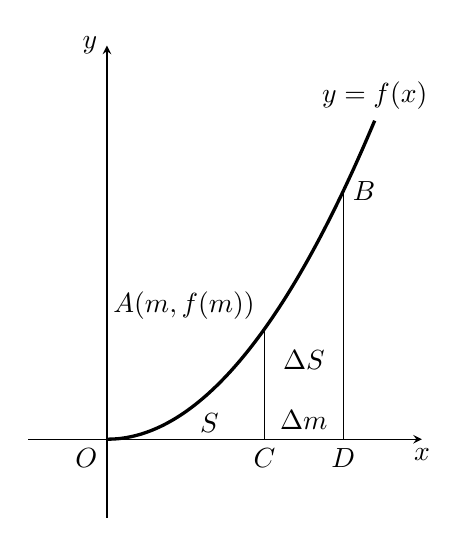
\begin{tikzpicture}[>=stealth, scale=2]
\draw[->](-.5,0)--(2,0)node[below]{$x$};    
\draw[->](0,-.5)--(0,2.5)node[left]{$y$};    
\draw[domain=0:1.7, very thick, smooth]plot(\x, {.7*\x^2})node[above]{$y=f(x)$};
\draw(1,0)node[below]{$C$}--(1,.7)node[above left]{$A(m,f(m))$};
\draw(1.5,0)node[below]{$D$}--(1.5,1.575)node[right]{$B$};
\node at (.65,.1){$S$};
\node at (1.25,.5){$\Delta S$};
\tkzDefPoints{0/0/O, 1.5/1.575/B, 1.5/0/D, 1/.7/A, 1/0/C}
\tkzMarkRightAngle[size=.1](A,C,O)
\node at (1.25,0)[above]{$\Delta m$};
\node [below left]{$O$};
\end{tikzpicture}
\captionof{figure}{}
\end{minipage}


\begin{solution}
\begin{enumerate}[(1)]
    \item 函数$g(m)$从$m$到$m+\Delta m$之间的平均变化率为
\[\begin{split}
\frac{\Delta S}{\Delta m}=\frac{g(m+\Delta m)-g(m)}{\Delta m}&=\frac{\frac{1}{2}(m+\Delta m)^3-\frac{1}{2}m^3}{\Delta m}\\
&=\frac{\frac{3}{2}m^2\cdot \Delta m+\frac{3}{2}m\cdot (\Delta m)^2+\frac{1}{2}(\Delta m)^3}{\Delta m}\\
&=\frac{3}{2}m^2+\frac{3}{2}m\cdot \Delta m+\frac{1}{2}(\Delta m)^2
\end{split}\]

\item $\Lim{\Delta m}{0}\frac{\Delta S}{\Delta m}=\Lim{\Delta m}{0}\left[\frac{3}{2}m^2+\frac{3}{2}m\cdot \Delta m+\frac{1}{2}(\Delta m)^2\right]=\frac{3}{2}m^2$

\item  当$|\Delta m|$充分小时,曲边梯形$ACDB$的面积$\Delta S$可用梯形$ACDB$的面积表示它的近似值,即$\Delta S\approx S_{\text{梯形}ACDB}$,因此$\frac{\Delta S}{\Delta m}\approx \text{梯形}ACDB$的中位线的长,

$\therefore\quad \Lim{\Delta m}{0}\frac{\Delta S}{\Delta m}=f(m)$,
即$f(m)=\frac{3}{2}m^2$.
\end{enumerate}
\end{solution}

\begin{ex}
\begin{enumerate}
    \item 已知函数$y=f(x)=x^2-x+2$的图象上有一动点$Q(x,y)$及定点$P(2,4)$.
\begin{enumerate}[(1)]
    \item 根据下表中$x_Q$的值,分别求出$f(x)$从2到$x_Q$之间的平均变化率;
\begin{center}
\begin{tabular}{c|ccccccc}
\hline
$x_Q$ & 4&3&2.5&2.1& 2.01& 2.001& 2.0001\\
\hline
$\Delta x$ \\
$\Delta y$ \\ [1.5ex]
$\frac{\Delta y}{\Delta x}$\\
\hline
\end{tabular}
\end{center}
\item 计算$\frac{f(2+\Delta x)-f(2)}{\Delta x}$
\item 计算$\Lim{\Delta x}{0}\frac{f(2+\Delta x)-f(2)}{\Delta x}$
\end{enumerate}

\item 对于12.1节中例12.1,计算$\Lim{\Delta t}{0}\frac{\Delta S}{\Delta t}$,并指出这个极限值的物理意义.
\item 已知$f(x)=\sqrt{25-x^2}$
\begin{enumerate}[(1)]
\item 计算$\frac{f(3+\Delta x)-f(3)}{\Delta x}$;
\item 计算$\Lim{\Delta x}{0}\frac{f(3+\Delta x)-f(3)}{\Delta x}$;
\item 试给出(2)中极限值的一种几何意义.
\end{enumerate}
\end{enumerate}
\end{ex}

\section{导数}
我们在研究函数$y=f(x)$的变量之间的关系时,不仅要
注意$f(x)$在$x_0$到$x_0+\Delta x$这一范围内的平均变化率,而且还要进一步研究当$\Delta x\to 0$时,$f(x)$在点$x=x_0$处的瞬时变化率. 例如,作非匀速直线运动的物体在某一时刻的瞬时速度;物体受热时,在某时刻温度的变化速度;导线在某时刻的电流强度;物质进行化学反应时,在某时刻的反应速度等.

设函数$y=f(x)$在点$x=x_0$及其附近有定义,$\Delta x$是自变量在点$x_0$的改变量,$\Delta y=f(x_0+\Delta x)-f(x_0)$是函数$f(x)$相应的改变量,若极限
\[\lim_{\Delta x\to 0}\frac{\Delta y}{\Delta x}=\lim_{\Delta x\to 0}\frac{f(x_0+\Delta x)-f(x_0)}{\Delta x}\]
存在,则称函数$f(x)$在点$x_0$处可导,且称此极限值为函数$f(x)$在点$x_0$的导数(即瞬时变化率,简称变化率),记作$f'(x_0)$或$y'\Big|_{x=x_0}$,于是
\[f'(x_0)=\lim_{\Delta x\to 0}\frac{\Delta y}{\Delta x}=\lim_{\Delta x\to 0}\frac{f(x_0+\Delta x)-f(x_0)}{\Delta x}\]

函数$f(x)$在点$x_0$处的导数$f'(x_0)$就是函数的平均变化率当$\Delta x\to 0$时的极限值,若极限值不存在,则称函数$f(x)$在点$x_0$处\textbf{不可导},即$f'(x_0)$不存在. 

若令$x=x_0+\Delta x$,代入上式,得
\[f'(x_0)=\lim_{x\to x_0}\frac{f(x)-f(x_0)}{x- x_0}\]
这是求$f'(x_0)$常用的另一种表达式.


\begin{example}
    已知$f(x)=\sqrt{x}$,求$f'(1)$, $f'(2)$
\end{example}

\begin{solution}
\[\begin{split}
f'(1)&=\Lim{x}{1}\frac{f(x)-f(1)}{x-1}=\Lim{x}{1}\frac{\sqrt{x}-1}{x-1}\\
&=\Lim{x}{1}\frac{\sqrt{x}-1}{(\sqrt{x}-1)(\sqrt{x}+1)}=\Lim{x}{1}\frac{1}{\sqrt{x}+1}=\frac{1}{2}\\
f'(2)&=\Lim{\Delta x}{0}\frac{f(2+\Delta x)-f(2)}{\Delta x}=\Lim{\Delta x}{0}\frac{\sqrt{2+\Delta x}-\sqrt{2}}{\Delta x}\\
&=\Lim{\Delta x}{0}\frac{\Delta x}{\Delta x\left(\sqrt{2+\Delta x}+\sqrt{2}\right)}\\
&=\Lim{\Delta x}{0}\frac{1}{\sqrt{2+\Delta x}+\sqrt{2}}=\frac{1}{2\sqrt{2}}
\end{split}\]
$\therefore\quad f'(1)=\frac{1}{2},\quad f'(2)=\frac{\sqrt{2}}{4}$
\end{solution}

\begin{example}
已知$f(x)=|x|$,求$f'(-1)$,$f'(0)$
\end{example}

\begin{solution}
\[\begin{split}
    f'(-1)&=\Lim{x}{-1}\frac{f(x)-f(-1)}{x-(-1)}= \Lim{x}{-1}\frac{|x|-1}{x+1}\\
    &=\Lim{x}{-1}\frac{-(x+1)}{x+1}=\Lim{x}{-1}(-1)=-1
\end{split} \]
$\therefore\quad f'(-1)=-1$

当$x\to 0$时,$\frac{\Delta y}{\Delta x}=\frac{|\Delta x|}{\Delta x}$

$\because\quad $当$\Delta x>0$时,$\frac{|\Delta x|}{\Delta x}=1$;当$\Delta x<0$时,$\frac{|\Delta x|}{\Delta x}=-1$

$\therefore\quad \Lim{\Delta x}{0}\frac{\Delta y}{\Delta x}=\Lim{\Delta x}{0}\frac{|\Delta x|}{\Delta x}$不存在,即$f(x)=|x|$在$x=0$时没有导数,$f'(0)$不存在.
\end{solution}

\begin{ex}
\begin{enumerate}
    \item 求$f'(2)$
\begin{multicols}{2}
\begin{enumerate}[(1)]
    \item $f(x)=x^3$
    \item $f(x)=\frac{1}{x}$
    \item $f(x)=-2x^2+3x+1$
\end{enumerate}
\end{multicols}
    \item 已知$f(x)=\sin x$,求:$f'\left(\frac{\pi}{6}\right)$、$f'\left(\frac{\pi}{2}\right)$
\end{enumerate}
\end{ex}

\section{导数的几何意义}
在12.1节中我们已经知道,若点$Q(x_0+\Delta x,y_0+\Delta y)$、$P(x_0,y_0)$分别是函数$y=f(x)$的图象上的两点,则割线的斜率为
\[K_{PQ}=\frac{\Delta y}{\Delta x}=\frac{f(x_0+\Delta x)-f(x_0)}{\Delta x}\]

若函数$f(x)$在点$x_0$处可导,则
\[f'(x_0)=\lim_{\Delta x\to 0}\frac{\Delta y}{\Delta x}=\lim_{\Delta x\to 0}\frac{f(x_0+\Delta x)-f(x_0)}{\Delta x}\]

当$\Delta x\to 0$时,如图12.3,点$Q(x_0+\Delta x,y_0+\Delta y)$沿着函数
$y=f(x)$的图象无限地趋近于$P(x_0,y_0)$点,这时割线$PQ$绕着点$P$转动,它的极限位置是函数$y=f(x)$的图象在点$P$处的切线. 因此,
\[K_{PT}=\lim_{Q\to P}K_{PQ}=\lim_{\Delta x\to 0}\frac{\Delta y}{\Delta x}=f'(x_0)\]

\begin{figure}[htp]
    \centering
\begin{tikzpicture}[>=stealth, scale=1.5]
\draw[->](-.75,0)--(5,0)node[right]{$x$};
\draw[->](0,-1)--(0,3.5)node[left]{$y$};
\draw[domain=-.5:4.75, very thick, samples=100, smooth]plot(\x, {.15*(1*\x+.5)*(1*\x-2)*(1*\x-4)+1.5})node[left]{$y=f(x)$};
\tkzDefPoints{3.5/1.05/P, 4.25/1.9/Q}
\tkzDrawLines[add= 2.5  and .75](P,Q)
\tkzLabelPoints[above](P)
\tkzLabelPoints[above left](Q)
\draw(4.25,1.06)--node[below]{$\Delta x$}(P)--(3.5,0)node[below]{$x_0$};
\draw(Q)--(4.25,0)node[below]{$x_0+\Delta x$};
\node [below left]{$O$};
\tkzDefPoints{3.5/0/A, 4.25/0/B, 4.25/1.05/S,0/0/O}
\tkzMarkRightAngles[size=.1](Q,S,P Q,B,A P,A,O)
\tkzLabelPoints[right](S)

\tkzDefPoints{4.25/1.7/Q1, 4.25/1.6/Q2, 4.25/1.5/Q3, 4.25/1.4/Q4}

\foreach \x in {1,2,3}
{
    \tkzDrawLines[add= 3  and .75](P,Q\x)
}

\tkzDrawLines[add= 4.5  and .75, very thick](P,Q4)
\node at (4.75,1.65)[right]{$T$};

\end{tikzpicture}
    \caption{}
\end{figure}

综上所述,函数$y=f(x)$在
点$x_0$处的导数$f'(x_0)$的几何意
义是曲线$y=f(x)$在点$(x_0,f(x_0))$处的切线的斜率.

\begin{example}
求与曲线$y=x^3$相切于点$A(-1,-1)$的切线方程,并作图.
\end{example}

\noindent
\begin{minipage}{.55\textwidth}
    \begin{analyze}
        欲求以点$A(-1,-1)$为切点的切线方程,只需求出切线的斜率,而$K_{\text{切}}=f'(-1)$.
    \end{analyze}
    
    \begin{solution}
\[\begin{split}
    K_{\text{切}}=f'(-1)&=\lim_{x\to -1}\frac{f(x)-f(-1)}{x-(-1)}\\
    &=\lim_{x\to -1}\frac{x^3+1}{x+1}\\
    &=\lim_{x\to -1}(x^2-x+1)=3
\end{split}\]
\[\begin{split}
    y-(-1)&=3[x-(-1)]\\
    y+1&=3x+3
\end{split}\]
$\therefore\quad y=3x+2$为所求的切线方程. 

作图如图12.4.    
\end{solution}
\end{minipage}
\begin{minipage}{.4\textwidth}
\centering
\begin{tikzpicture}[>=stealth, scale=.5]
\draw[->](-4,0)--(5,0)node[below]{$x$};    
\draw[->](0,-3)--(0,10)node[left]{$y$};
\draw[domain=-1.3:2.1, smooth, very thick, samples=100]plot(\x, {\x^3});
\node[below right]{$O$};
\tkzDefPoints{-1/-1/A, 2/8./B}
\tkzDrawLines[](A,B)
\node at (A)[left] {$A(-1,-1)$};
\node at (B)[right] {$B(2,8)$};
\tkzDrawPoints(A,B)
\node at (-.25,1.25)[left]{$y=3x+2$};
\node at (1.5,3.375)[right]{$y=x^3$};
\end{tikzpicture}
\captionof{figure}{}
\end{minipage}
    
\begin{example}
求过曲线$y^2=2px\; (y\ge 0)$上一点$P(x_0,y_0)$的切线方程.
\end{example}

\begin{solution}
$y=\sqrt{2px}\quad (y\ge 0,\; x\ge 0)$
\[\begin{split}
    y' \Big|_{x=x_{0}}=\lim_{x\to x_{0}}\frac{\sqrt{2px}-\sqrt{2px_{0}}}{x-x_{0}}&=\lim_{x\to x_{0}}\frac{\sqrt{2p}(\sqrt{x}-\sqrt{x_{0}})}{(\sqrt{x}-\sqrt{x_{0}})(\sqrt{x}+\sqrt{x_{0}})}\\
    &=\lim_{x\to x_{0}}\frac{\sqrt{2p}}{\sqrt{x}+\sqrt{x_{0}}}=\sqrt{\frac{p}{2x_{0}}}\\
\end{split}\]
以$P(x_0,y_0)$为切点做切线方程为
\[\begin{split}
    y-y_0&=\sqrt{\frac{p}{2x_0}}(x-x_0)\\
    y-\sqrt{2px_0}&=\sqrt{\frac{p}{2x_0}}x-\sqrt{\frac{px_0}{2}}\\
y&=\sqrt{\frac p{2x_{0}}}x+\sqrt{\frac{px_{0}}2}=\frac{p}{\sqrt{2px_{0}}}(x+x_{0})
\end{split}\]
$\therefore\quad y_{0}y= p( x+ x_{0})$为所求切线方程.
\end{solution}

\begin{ex}
\begin{enumerate}
    \item 已知曲线$y=x^2-x$,分别求出在下列点处的切线方程:
\begin{multicols}{2}
\begin{enumerate}[(1)]
    \item $A(1,0)$
    \item $B(0,0)$
\end{enumerate}
\end{multicols}
    \item 求曲线$y=6x^{-1}$在点$A(3,2)$处的切线方程.
    \item 若函数$f(x)$在点$x_0$处及其附近可导,当$|\Delta x|$很小时,$\Delta y\approx$\blank .
\end{enumerate}
\end{ex}

\section{函数可导与连续的关系}
由12.2节中的例12.4可知,函数$f(x)=|x|$在$x=0$时连续,但$f'(0)$不存在.因此.若函数$f(x)$在点$x_0$处连续,函数$f(x)$在该点不一定可导. 反过来,若函数$f(x)$在点$x_0$处可导,则可以证明函数$f(x)$在该点一定连续. 事实上,欲证$f(x)$在点$x_0$处连续,只需证
$\Lim{x}{x_0}f(x)=f(x_0)$.

\[\begin{split}
\because\quad \Lim{x}{x_0}f(x)&=\Lim{x}{x_0}[f(x)-f(x_0)+f(x_0)]=\Lim{x}{x_0}[f(x)-f(x_0)]+f(x_0)\\
&=\Lim{x}{x_0}\left[\frac{f(x)-f(x_0)}{x-x_0}\cdot (x-x_0)\right]+f(x_0)\\
&=\Lim{x}{x_0} \frac{f(x)-f(x_0)}{x-x_0}  \cdot \Lim{x}{x_0}(x-x_0)+f(x_0)\\
&=f'(x_0)\cdot 0+f(x_0) =f(x_0)
\end{split}\]

$\therefore\quad \Lim{x}{x_0}f(x)=f(x_0)$即$f(x)$在点$x_0$处连续.

\begin{thm}{定理}
    若函数$f(x)$在点$x_0$处可导,则函数$f(x)$在点$x_0$处也连续.
\end{thm}

\begin{example}
    已知 函数$f(x)=|x^2-1|$
\begin{enumerate}[(1)]
\item 函数在$x_1=-1,\; x_2=0,\; x_3=-1$是否连续?
\item 函数在$x_1=-1,\; x_2=0,\; x_3=-1$是否可导?
\end{enumerate}
\end{example}

\begin{solution}
\[f(x)=|x^2-1|=\begin{cases}
    x^2-1,& x\le -1\; \text{或}\; x\ge 1\\
    1-x^2,& -1\le x\le 1
\end{cases}\]
\begin{enumerate}[(1)]
    \item $\because\quad \Lim{x}{0}f(x)=\Lim{x}{0}(1-x^2)=1=f(0)$

    $\therefore\quad f(x)$在$x=0$处连续.

$\because\quad \Lim{x}{1^+}f(x)=\Lim{x}{1^+}(x^2-1)=0,\;  \Lim{x}{1^-}f(x)=\Lim{x}{1^-}(1-x^2)=0,\; f(1)=0$

$\therefore\quad f(x)$在$x=1$处连续. 同理可证$f(x)$在$x=-1$处连续.

\item $\because\quad \Lim{x}{0}\frac{f(x)-f(0)}{x}=\Lim{x}{0}\frac{1-x^2-1}{x}=\Lim{x}{0}(-x)=0$

$\therefore\quad f'(0)$存在,且$f'(0)=0$
\[\begin{split}
  \because\quad  \Lim{x}{1^+}\frac{f(x)-f(1)}{x-1}&= \Lim{x}{1^+}\frac{x^2-1}{x-1}= \Lim{x}{1^+}(x+1)=2\\
  \Lim{x}{1^-}\frac{f(x)-f(1)}{x-1}&=\Lim{x}{1^-}\frac{1-x^2}{x-1}=-\Lim{x}{1^-}(x+1)=-2
\end{split}\]
$\therefore\quad f(x)$在$x=1$处不可导. 同理可证,$f(x)$在$x=-1$处也不可导.
\end{enumerate}
\end{solution}

\begin{ex}
\begin{enumerate}
    \item 作函数$y=|x^2-x|$的图象,并说明它在哪个点不可导.
    \item 已知函数$f(x)=\begin{cases}
        x\sin\frac{1}{x},& x\ne 0\\
        0,& x=0
    \end{cases}$

    试说明此函数$f(x)$在点$x=0$处是否可导及连续.
\end{enumerate}
\end{ex}

\section*{习题一}
\begin{center}
    \bfseries A
\end{center}

\begin{enumerate}
    \item 分别求下列函数的平均变化率$\frac{\Delta y}{\Delta x}$:
\begin{enumerate}[(1)]
    \item $y=-2x^3+x^2-1$,当$x=1$, $\Delta x=0.1$时;
    \item $y=\frac{x}{3}$,当$x=2$, $\Delta x=0.01$时;
    \item $y=\sqrt{2x}$,当$x=4$, $\Delta x=0.001$时.
\end{enumerate}
    ((2)、(3)题精确到0.001)
    \item     根据导数定义,求下列函数在给定点的导数:
\begin{multicols}{2}
\begin{enumerate}[(1)]
    \item $y=-2x^3+x^2-1$,求$f'(1)$;
    \item $y=\frac{3}{x}$,求$f'(2)$;
    \item $y=\sqrt{2x}$,求$f'(4)$.
\end{enumerate}
\end{multicols}
    \item    一质点做直线运动,它所经过的路程和时间的关系是$s=3t^2+2t+1$,求$t=2$时的瞬时速度.
    \item    求曲线$y=x^3$在点$A(2,8)$处的切线方程.
\end{enumerate}

\begin{center}
    \bfseries B
\end{center}

\begin{enumerate}\setcounter{enumi}{4}
    \item 已知$f(x)=\begin{cases}
        x^2\sin\frac{1}{x},& x\ne 0\\
        0,& x=0
    \end{cases}$,求$f'(0)$.
\item 函数$y=|\sin x|$在$x=0$处是否存在导数?并说明你的理由.
\item 已知$f(x)=\begin{cases}
    2x^2,& x\le 1\\
-2x^2+8x-4,& x\ge 1
\end{cases}$
,求$f'(1)$
\item 设$f(x)$在点$x=1$处的导数为$f'(1)$,计算
\begin{multicols}{2}
\begin{enumerate}[(1)]
    \item $\Lim{h}{0}\frac{f(1+3h)-f(1)}{h}$
    \item $\Lim{h}{0}\frac{f(1+h)-f(1-h)}{2h}$
\end{enumerate}
\end{multicols}
\end{enumerate}

\section*{二、函数的导数}

\section{函数的导数}

我们已经学了函数$f(x)$在点$x_0$处的导数,例如$f(x)=\frac{1}{x}$在点$x_0$处的导数为:
\[\begin{split}
f'(x_0)&=\Lim{h}{0}\frac{f(x_0+h)-f(x_0)}{h}=\Lim{h}{0}\frac{\frac{1}{x_0+h}-\frac{1}{x_0}}{h}\\
&=\Lim{h}{0}\frac{x_0-(x_0+h)}{hx_0(x_0+h)}=\Lim{h}{0}\frac{-1}{x_0(x_0+h)}=-\frac{1}{x^2_0}
\end{split}\]
即:$f'(x_0)=-\frac{1}{x^2_0}$

如果$x_0\in (0,+\infty)$,不难看出,对于开区间$(0,+\infty)$内每一个确定的值$x_0$,都有唯一确定的值$f'(x_0)$与其相对应,这样,在开区间$(0,+\infty)$内,利用求导的方法又得到了一个新
的函数$f'(x)=-\frac{1}{x^2}$.

一般地,若函数$f(x)$在开区间$(a,b)$内每一点$x$处都可导,即.
\[f'(x)=\Lim{h}{0}\frac{f(x+h)-f(x)}{h}\qquad x\in(a,b)\]
则由此对应法则确定的函数$f'(x)$叫做函数$f(x)$的导函数(简称$f(x)$的导数)。这时又称$f(x)$在开区间$(a,b)$内可导.

下面根据函数的导数定义,求几种最常见的函数的导数.
\begin{enumerate}
    \item $f(x)=c$($c$为常数)的导数.

    $\because\quad f'(x)=\Lim{h}{0}\frac{f(x+h)-f(x)}{h}=\Lim{h}{0}\frac{c-c}{h}=0$

$\therefore\quad    f'(x)=c'=0$($c$为常数).
    \item $f(x)=x^n$($n$为自然数)的导数.
\[\begin{split}
    \because\quad f'(x)&=\Lim{h}{0}\frac{f(x+h)-f(x)}{h}=\Lim{h}{0}\frac{(x+h)^n-x^n}{h}\\
&=\Lim{h}{0}\left({\rm C}^1_n x^{n-1}+{\rm C}^2_nx^{n-2}\cdot h+\cdots+{\rm C}^k_nx^{n-k}\cdot h^{k-1}+\cdots +h^{n-1}\right)\\
&={\rm C}^1_nx^{n-1}=nx^{n-1}
\end{split}\]
$\therefore\quad f'(x)=(x^n)'=nx^{x-1}$($n$为自然数).
    \item $f(x)=\sin x$的导数.
    \[\begin{split}
        \because\quad f'(x)&=\Lim{h}{0}\frac{f(x+h)-f(x)}{h}=\Lim{h}{0}\frac{\sin (x+h)-\sin x}{h}\\
    &=\Lim{h}{0}\frac{2\cos \left(x+\frac{h}{2}\right)\sin \frac{h}{2}}{h}\\
    &=\Lim{h}{0}\cos \left(x+\frac{h}{2}\right)\cdot \Lim{\tfrac{h}{2}}{0}\frac{\sin\frac{h}{2}}{\frac{h}{2}}=\cos x
    \end{split}\]
    $\therefore\quad f'(x)=(\sin x)'=\cos x$.

\item $f(x)=\cos x$的导数.
\[\begin{split}
    \because\quad f'(x)&=\Lim{h}{0}\frac{f(x+h)-f(x)}{h}=\Lim{h}{0}\frac{\cos (x+h)-\cos x}{h}\\
&=\Lim{h}{0}\frac{-2\sin \left(x+\frac{h}{2}\right)\sin \frac{h}{2}}{h}\\
&=-\Lim{h}{0}\sin \left(x+\frac{h}{2}\right)\cdot \Lim{\tfrac{h}{2}}{0}\frac{\sin\frac{h}{2}}{\frac{h}{2}}=-\sin x
\end{split}\]
$\therefore\quad f'(x)=(\cos x)'=-\sin x$.

\item $f(x)=\ln x$的导数.
\[\begin{split}
    \because\quad f'(x)&=\Lim{h}{0}\frac{f(x+h)-f(x)}{h}=\Lim{h}{0}\frac{\ln (x+h)-\ln x}{h}\\
&=\Lim{h}{0}\frac{1}{h}\ln\left(1+\frac{h}{x}\right)=\Lim{h}{0}\left[\frac{1}{x}\cdot \frac{x}{h}\ln\left(1+\frac{1}{\frac{x}{h}}\right)\right]\\
&=\frac{1}{x}\lim_{\tfrac{x}{h}\to \infty}\ln\left(1+\frac{1}{\frac{x}{n}}\right)^{\tfrac{x}{h}}=\frac{1}{x}\ln\left[\lim_{\tfrac{x}{h}\to\infty}\left(1+\frac{1}{\frac{x}{h}}\right)^{\tfrac{x}{h}}\right]\\
&=\frac{1}{x}\ln e=\frac{1}{x}
\end{split}\]
$\therefore\quad f'(x)=(\ln x)'=\frac{1}{x},\quad (x>0)$.
\end{enumerate}

综上所述,目前我们得到几种最常见的函数的导数为(今后可当公式用):
\begin{thm}{}
   \begin{enumerate}
\item $c'=0$($c$为常数).
\item $(x^n)'=nx^{n-1}$($n$为自然数).
\item $(\sin x)'=\cos x$.
\item $(\cos x)'=-\sin x$.
\item $(\ln x)'=\frac{1}{x}$
\end{enumerate}     
\end{thm}

\begin{ex}
\begin{enumerate}
    \item 求下列函数的导数:
\begin{multicols}{2}
\begin{enumerate}[(1)]
\item $f(x)=x^{10}$;
\item $f(x)=x^{99}$;
\item $f(x)=\cos x$;
\item $f(x)=\ln x$.
\end{enumerate}
\end{multicols}
    \item 根据函数的导数定义,求下列函数的导数.
\begin{multicols}{2}
\begin{enumerate}[(1)]
\item $f(x)=3x^4+2x^3$;
\item $f(x)=\frac{1}{x^2}$;
\item $f(x)=\sqrt{x}$;
\item $f(x)=\sin3x$;
\item $f(x)=\cos(-2x)$.
\end{enumerate}
\end{multicols}
\end{enumerate}
\end{ex}

\section{函数的和、差、积、商的导数}
如同研究函数极限的四则运算一样,下面研究函数的四则运算的导数.

已知函数$f(x)$、$g(x)$的导数分别为$f'(x)$、$g'(x)$

\subsection{$y=f(x)+g(x)$}
\[\begin{split}
    \because\quad y' &=\lim_{\Delta x\to0}\frac{\Delta y}{\Delta x}=\lim_{\Delta x\to0}\frac{\left[f(x+\Delta x)+g(x+\Delta x)\right]-\left[f(x)+g(x)\right]}{\Delta x}\\
    &=\lim_{\Delta x\to0}\left[\frac{f(x+\Delta x)-f(x)}{\Delta x}+\frac{g(x+\Delta x)-g(x)}{\Delta x}\right]\\
    &=\lim_{\Delta x\to0}\frac{f(x+\Delta x)-f(x)}{\Delta x}+\lim_{\Delta x\to0}\frac{g(x+\Delta x)-g(x)}{\Delta x}\\
    &=f' (x)+g' (x)
\end{split}\]

$\therefore\quad y' =[f(x)+g(x)]' =f' (x)+g' (x)$

\begin{thm}{定理1}
\[[f(x)+g(x)]' =f' (x)+g' (x)\]
\end{thm}

\begin{thm}{推论}
\[[f(x)-g(x)]' =f' (x)-g' (x)\]
\end{thm}

\subsection{ $y=f(x)g(x)$}
\[\begin{split}
\because\quad \Delta y=&f(x+\Delta x)g(x+\Delta x)-f(x)g(x)\\
&=f(x+\Delta x)g(x+\Delta x)-f(x)g(x+\Delta x)+f(x)g(x+\Delta x)-f(x)g(x)\\
&=[f(x+\Delta x)-f(x)]g(x+\Delta x) +f(x)[g(x+\Delta x)-g(x)]
\end{split}\]
而
\[\begin{split}
    y' &=\lim_{\Delta x\to0}\frac{\Delta y}{\Delta x}=\lim_{\Delta x\to0}\frac{\left[f(x+\Delta x)-f(x)\right]g(x+\Delta x)+f(x)\left[g(x+\Delta x)-g(x)\right]}{\Delta x}\\
    &=\lim_{\Delta x\to0}\frac{f(x+\Delta x)-f(x)}{\Delta x}\cdot\lim_{\Delta x\to0}g(x+\Delta x)+f(x)\cdot\lim_{\Delta x\to0}\frac{g(x+\Delta x)-g(x)}{\Delta x}\\
    &=f' (x)g(x)+f(x)g' (x)
\end{split}\]

$\therefore\quad y' =[f(x)g(x)]' =f' (x)g(x)+f(x)g' (x)$

\begin{thm}{定理2}
\[[f(x)g(x)]' =f' (x)g(x)+f(x)g' (x)\]
\end{thm}

\begin{thm}{推论}
   \[ [cf(x)]'=cf'(x)\qquad \text{($c$为常数)}\]
\end{thm}

\begin{example}
求下列函数的导数
\begin{multicols}{2}
\begin{enumerate}[(1)]
    \item $y=x^3+\sin x$
    \item $y=x^3\sin x$
\end{enumerate}
\end{multicols}
\end{example}

\begin{solution}
\begin{enumerate}[(1)]
    \item $y'=(x^3)'+(\sin x)'=3x^2+\cos x$

$\therefore\quad y'=3x^2+\cos x$

\item $y'=(x^3)'\sin x+x^3(\sin x)'=3x^2\sin x+x^3\cos x$

$\therefore\quad y'=3x^2\sin x+x^3\cos x$
 \end{enumerate}   
\end{solution}

\subsection{$y=\frac{f(x)}{g(x)}$}
\[\begin{split}
    \because\quad  y&=\frac{f(x)}{g(x)}=f(x)\cdot \frac{1}{g(x)}\\
y'&=f'(x)\cdot \frac{1}{g(x)}+f(x)\cdot \left[\frac{1}{g(x)}\right]'
\end{split}\]

$\therefore\quad $欲求$y'$,只需求出$\left[\frac{1}{g(x)}\right]'$

\[\begin{split}
  \because\quad   \left[\frac{1}{g(x)}\right]' &=\lim_{h\to 0}\frac{\frac{1}{g(x+h)}-\frac{1}{g(x)}}{h}=\lim_{h\to 0}\frac{g(x)-g(x+h)}{hg(x+h)g(x)}\\
    &=\frac{1}{g(x)}\cdot \lim_{h\to 0}\frac{-[g(x+h)-g(x)]}{h}\cdot \lim_{h\to 0}\frac{1}{g(x+h)}\\
&=\frac{1}{g(x)}\cdot [-g'(x)]\cdot \frac{1}{g(x)}=-\frac{g'(x)}{[g(x)]^2}
\end{split}\]
\[\begin{split}
    \therefore\quad \left[\frac{1}{g(x)}\right]' &=-\frac{g'(x)}{[g(x)]^2}\\
    y'=\left[\frac{f(x)}{g(x)}\right]'&=f' \left(x\right)\cdot\frac{1}{g\left(x\right)}+f\left(x\right)\cdot\left[\frac{1}{g\left(x\right)}\right]' \\
    &=f' \left(x\right)\cdot\frac{1}{g\left(x\right)}-f\left(x\right)\cdot\frac{g' \left(x\right)}{\left[g\left(x\right)\right]^{2}}\\
    &=\frac{f' \left(x\right)g\left(x\right)-f\left(x\right)g' \left(x\right)}{\left[g\left(x\right)\right]^{2}}
\end{split}\]

\begin{thm}{定理3}
\[\left[\frac{f(x)}{g(x)}\right]'=\frac{f' \left(x\right)g\left(x\right)-f\left(x\right)g' \left(x\right)}{\left[g\left(x\right)\right]^{2}}\]
其中$g(x)\ne 0$.
\end{thm}

\begin{example}
    求下列函数的导数
\begin{multicols}{2}
\begin{enumerate}[(1)]
    \item $y=\frac{x^3}{\sin x}$
    \item $y=\frac{1}{x^3}$
\end{enumerate}
\end{multicols}
\end{example}

\begin{solution}
\begin{enumerate}[(1)]
    \item $y'=\left(\frac{x^3}{\sin x}\right)'=\frac{(x^3)'\sin x-x^3 (\sin x)'}{\sin^2 x}=\frac{3x^2\sin x-x^3\cos x}{\sin^2 x}$
    
    $\therefore\quad y'=\frac{3x^2\sin x-x^3\cos x}{\sin^2 x}$
    \item $y'=\left(\frac{1}{x^3}\right)'=\frac{0\cdot x^3-1\cdot (x^3)'}{(x^3)^2}=-\frac{3x^2}{x^6}=-\frac{3}{x^4}$
\end{enumerate}    
\end{solution}

\begin{example}
    求证:当$n$为负整数时,公式$(x^n)'=nx^{n-1}$仍然成立.
\end{example}

\begin{proof}
设$n=-k$($k$为自然数)
\[\begin{split}
 \because\quad (x^n)'=\left(\frac{1}{x^k}\right)'=\frac{0\cdot x^k-1\cdot (x^k)'}{(x^k)^2}&=-\frac{kx^{k-1}}{x^{2k}}\\
 &=\frac{-k}{x^{k+1}}=-kx^{-(k+1)}=nx^{n-1}   
\end{split}\]

$\therefore\quad (x^n)'=nx^{n-1}$($n$为负整数).
\end{proof}


\begin{rmk}
\begin{enumerate}
    \item 由例12.10可知,公式$(x^n)'=nx^{n-1}$可由$n$为自然数推广到$n$为任意整数.
    \item 若$f(x)$、$g(x)$可导,则$f(x)\pm g(x)$、$f(x)g(x)$、$\frac{f(x)}{g(x)}\; (g(x)\ne 0)$都可导,并且
\begin{enumerate}[(1)]
\item $[f(x)\pm g(x)]'=f'(x)\pm g'(x)$;
\item $[f(x)g(x)]'=f'(x)g(x)+f(x)g'(x)$;
\item $\left[\frac{f(x)}{g(x)}\right]'=\frac{f'(x)g(x)-f(x)g'(x)}{[g(x)]^2}$.
\end{enumerate}

    \item 利用数学归纳法,不难得出
\[ [f_1(x)+f_2(x)+\cdots +f_n(x)]'=f'_1(x)+f'_2(x)+\cdots +f'_n(x)\]
    对于$[f_1(x)f_2(x)\cdots f_n(x)]'=?$ 留给读者去证明自己的猜想.
    \item 利用上述函数四则运算的导数公式,可将某些初等函数的导数问题转化为最简单的函数的导数来解决.
\end{enumerate}
\end{rmk}


\begin{ex}
\begin{enumerate}
    \item 求下列各函数的导数:
\begin{enumerate}[(1)]
    \item $3x^4-4x^3+6x^2-7x+100-3x^{-1}+5x^{-2}-6x^{-3}$;
    \item $x\ln x$;
    \item $(3x^2+1)(x+\cos x)$;
    \item $\frac{2x-1}{x+1}$.
\end{enumerate}
    \item 求下列函数的导数(今后可当公式用):
\begin{multicols}{2}
\begin{enumerate}[(1)]
    \item $\tan x$
    \item $\cot x$
    \item $\sec x$
    \item $\csc x$
\end{enumerate}
\end{multicols}
\end{enumerate}
\end{ex}

\section*{习题二}
\begin{center}
    \bfseries A
\end{center}

\begin{enumerate}
    \item 求下列函数的导数:
\begin{multicols}{2}
\begin{enumerate}[(1)]
    \item $- 3x^{2}+ 2x+ 1$
    \item $( x+ 1) ^{2}( x- 1)$
    \item $\frac{x+1}{x-1}$
    \item $\frac{1}{x^{2}-3x+6}$
    \item $x\sin x+\cos x$
    \item $\frac{\sin x}{1+\cos x}$
    \item $\frac{\ln x}{x}$
    \item $x\tan x-\cot x$
\end{enumerate}    
\end{multicols}
\item 已知:$f(x)=\cos x-\sin x$ 求:$f' \left(\frac\pi3\right)$, $f' \left(\frac{3\pi}4\right)$.
\item 已知:$f(x)=\frac{3}{5-x}+\frac{x^{2}}{5}$, 求:$f' (0)$, $f' (2)$.
\end{enumerate}

\begin{center}
    \bfseries B
\end{center}

\begin{enumerate}\setcounter{enumi}{3}
    \item 求下列函数的导数:
    \begin{multicols}{2}
    \begin{enumerate}[(1)]
\item $x^{2}\tan x$
\item $\frac{x^{2}}{\tan x}$
\item $\frac{\cos x}{1-x^{2}}$
\item $x\sin x\ln x$
\item $x\tan x-\cot x$
\item $(x-a)(x-b)(x-c)$
    \end{enumerate}    
\end{multicols}

\item 设$f(x)=\frac{x^{3}}{3}+\frac{x^{2}}{2}-2x$, 求下列方程的解集:
\begin{multicols}{3}
\begin{enumerate}[(1)]
    \item $f' (x)=0$
    \item $f' (x)=-2$
    \item $f' (x)=10$
\end{enumerate}
\end{multicols}

\item 设$f(x+1)=x^{3}-1$, 求$f' (x)$.
\item 设$f(x)=\begin{cases}
    3-x,& x<1\\
    (3-x)(1-x),& 1\le x<2\\
    -(1-x),& x\ge 2
\end{cases}$,求$f'(x)$.
\item 已知$f(x)=x\sin x$.
\begin{enumerate}[(1)]
\item 求$f'(x)$;
\item 若令$F(x)=f'(x)$,求$F'(x)$.
\end{enumerate}

\item 已知$f(x)=(5x+2)^4$,求$f'(x)$.
\end{enumerate}

\section{复合函数的导数}
在求函数$f(x)=(5x+2)^4$的导数$f'(x)$时,可将
$(5x+2)^4$“展开”后再求导,也可运用函数乘积的导数运算定理求. 即
\[\begin{split}
[(5x+2)^{4}]' &=(5x+2)' (5x+2)^{3}+(5x+2)[(5x+2)^{3}]' \\
&=(5x+2)' (5x+2)^{3}+(5x+2)' (5x+2)^{3}+(5x+2)^{2}[(5x+2)^{2}]' \\
&=2(5x+2)' (5x+2)^{3}+(5x+2)^{2}[2(5x+2)' (5x+2)]\\
&=4(5x+2)^{3}(5x+2)'     
\end{split}\]
$\therefore\quad f' (x)=[(5x+2)^{4}]'=4(5x+2)^{3}(5x+2)=20(5x+2)^{3}$

由于函数$f(x)=(5x+2)^4$可以看成是由函数$y=u^4$和$u=5x+2$复合而成的. 从这个例子我们看到,函数$y=(5x+2)^4$的导数恰好等于对中间变量$u$的导数乘以中间变量对$x$的导数(即$4u^3\cdot u'_x$).

\begin{thm}
{定理} 由函数$y=f(u)$和$u=\varphi(x)$构成的复合函数$y=f[\varphi(x)]$对自变量$x$的导数$y'_x$等于$y$对中间变量$u$的导数$y'_u$ 乘以中间变量$u$对自变量$x$的导数$u'_x$,即
\[y'_x=y'_u\cdot u'_x\]    
\end{thm}

\begin{proof}
若函数$y=f(u)$在点$u$处可导,则
    $\Delta y=f' \left(u\right)\cdot \Delta u+\alpha\left(\Delta u\right)$(其中当$\Delta u\to0$时,$\alpha(\Delta u)\to0$)

\[\begin{split}
    \because\quad y'_x=\lim_{\Delta x\to0}\frac{\Delta y}{\Delta x}&=\lim_{\Delta x\to0}\frac{f' (u)\cdot\Delta u+\alpha(\Delta u)}{\Delta x}\\
    &=f' \left(u\right)\lim_{\Delta x\to0}\frac{\Delta u}{\Delta x}+\lim_{\Delta x\to0}\frac{\alpha\left(\Delta u\right)}{\Delta x}\\
    &=f(u)\varphi' (x)+0=y'_{u}\cdot  u'_{x}
\end{split}\]
$\therefore\quad y'_x=y'_{u}\cdot  u'_{x}$.
\end{proof}

\begin{rmk}
这个求复合函数导数的方法,可以推广到两个以上的中间变量.例如,若函数$y=f(x)$是由函数$y=h(u)$, $u=\varphi(t)$, $t=g(x)$复合而成的,则$y'_x=y'_u\cdot u'_t\cdot t'_x$.
\end{rmk}

在求复合函数的导数时,关键在于分析清楚该函数是由哪几个函数复合而成的,否则极容易出现计算错误,请读者特别注意.

\begin{example}
    求$y=\sin^2 3x$的导数.
\end{example}

\begin{analyze}
函数$y=\sin^2 3x$是由$y=u^2$, $u=\sin t$, $t=3x$复合而成的.
\end{analyze}

\begin{solution}
\textbf{解法1} 
\[\begin{split}
    \because\quad y'_x=y'_u\cdot u'_t\cdot t'_x &=(u^2)'_u\cdot (\sin t)'_t\cdot (3x)'\\
    &=2u\cdot \cos t\cdot 3 =6\sin 3x\cos 3x=3\sin 6x
\end{split}\]

$\therefore\quad y'_x=3\sin 6x$.

\textbf{解法2}
\[\begin{split}
    \because \quad y' _{x}=(\sin^{2}3x)' &=2\sin3x\cdot (\sin 3x)' \\
    &=2\sin 3x\mathrm{cos}3x\cdot (3x)' =\sin 6x\cdot 3 =3\sin 6x.
\end{split}\]

$\therefore\quad y'_x=3\sin 6x$.
\end{solution}

\begin{example}
    求函数$y=\frac{1}{(2-5x)^4}$的导数
\end{example}

\begin{analyze}
    函数$y=\frac{1}{(2-5x)^4}$是由函数$y=u^{-4}$, $u=2-5x$复合而成的.
\end{analyze}

\begin{solution}
    \textbf{解法1} 
\[\begin{split}
    \because\quad y'_x=y'_u\cdot u'_x &=(u^{-4})'_u\cdot (2-5x)'\\
    &=-4u^{-5}\cdot (-5) =20(2-5x)^{-5}=\frac{20}{(2-5x)^5}
\end{split}\]

$\therefore\quad y'_x=\frac{20}{(2-5x)^5}$.

\textbf{解法2}
\[\begin{split}
    \because \quad y' _{x}=[(2-5x)^{-4}]' &=-4(2-5x)^{-5}\cdot (2-5x)' \\
    &=\frac{-4}{(2-5x)^5}\cdot (-5)=\frac{20}{(2-5x)^5}
\end{split}\]

$\therefore\quad y'_x=\frac{20}{(2-5x)^5}$.
\end{solution}

\begin{example}
求函数$y=x^{\alpha}$ ($\alpha$为任意实数,$x\in\R^+$)的导数.
\end{example}

\begin{analyze}
    由于等式$y=x^{\alpha}$的右边是幂的形式且$x>0$,我们不妨对等式两边取对数.
\[\ln y=\alpha\ln x\]
这时等式两边就都能利用已有的知识对$x$求导了.
\end{analyze}

\begin{solution}
\[\begin{split}
    y&=x^{\alpha}\\
    \ln y&=\alpha\ln x\\
\frac{1}{y}\cdot y'_x &=\frac{\alpha}{x}\\
y'_x&=y\cdot\frac{\alpha}{x}=\frac{\alpha x^{\alpha}}{x}=\alpha x^{\alpha-1}
\end{split}\]
$\therefore\quad y'=\alpha x^{\alpha-1}$
\end{solution}

\begin{rmk}
\begin{enumerate}
    \item 例12.13最终解决了幂函数$x^{\alpha}$($\alpha$为任意实数,$x\in\R^+$)的导数.
\[    (x^{\alpha})'=\alpha x^{\alpha-1}\]
    作为它的特例,
\[\begin{split}
    (x^{n})'=n x^{n-1}&\qquad (n\in\Z)\\
    \left(\sqrt[n]{x}\right)'=\frac{1}{n\sqrt[n]{x^{n-1}}}&\qquad (n\in\Z\text{且}n\ge 2)\\
\end{split}\]

\item 欲求函数$y=f(x)$的导数,先将它的两边取对数,然后再对它的两边分别按复合函数求导,这对于能利用对数运算性质变形的一些函数来说,是可采用的一种求导方法. 例如,求指数函数$y=a^x\; (a>0\text{且}a\ne 1)$的导数.
\[\begin{split}
    \ln y&= x\ln a\\
    \frac{1}{y}\cdot y'_x&=\ln a\\
    y'_x&=y\ln a=a^x\ln a
\end{split}\]
$\therefore\quad (a^x)'=a^x\ln a$

特别地,当$a=e$时,$(e^x)'=e^x$.
\end{enumerate}
\end{rmk}




\begin{example}
    例4 求函数 $y= \sqrt [ 3] {\frac {x+ 2}{x- 1}}$ $( x> 1)$的导数


\end{example}

\begin{solution}
\textbf{解法1} 
\[\begin{split}
    \because\quad  y'=\left(\sqrt[3]{\frac{x+2}{x-1}}\right)' &=\frac{1}{3}\left(\frac{x+2}{x-1}\right)^{-\tfrac{2}{3}}\cdot\left(\frac{x+2}{x-1}\right)' \\
    &=\frac{1}{3}\left(\frac{x-1}{x+2}\right)^{\tfrac{2}{3}}\cdot\frac{-3}{(x-1)^{2}}=-\frac{\sqrt[3]{(x-1)^2(x+2)}}{(x-1)^2(x+2)}
\end{split}\]
$\therefore\quad y'=-\frac{\sqrt[3]{(x-1)^2(x+2)}}{(x-1)^2(x+2)}$

\textbf{解法2} $\because\quad y=\left(\sqrt[3]{\frac{x+2}{x-1}}\right)\quad (x>1)$

$\therefore\quad \ln y=\frac{1}{3}\left[\ln(x+2)-\ln(x-1)\right]$

两边对$x$求导,得
\[\begin{split}
    \frac{1}{y}\cdot y'_x&=\frac{1}{3}\left(\frac{1}{x+2}-\frac{1}{x-1}\right)\\
    y'_x&=\frac{y}{3}\cdot \frac{-3}{(x+2)(x-1)}=-\sqrt[3]{\frac{x+2}{x-1}}\cdot \frac{1}{(x+2)(x-1)}\\
    &=-\frac{\sqrt[3]{(x-1)^2(x+2)}}{(x-1)^2(x+2)}
\end{split} \]
即:$y'=-\frac{\sqrt[3]{(x-1)^2(x+2)}}{(x-1)^2(x+2)}$
\end{solution}

\begin{ex}
\begin{enumerate}
    \item 填空(写出下列函数$f(x)$的导数):
\begin{multicols}{2}
\begin{enumerate}[(1)]
    \item 若$c$为常数,则$c'=\blank$;
    \item $(x^{a})'=\blank$;
    \item $(a^x)'=\blank$;
    \item $\left(\frac{1}{x}\right)'=\blank$;
    \item $(\sqrt{x})'=\blank$;
    \item $(\ln x)'=\blank$;
    \item $(e^x)'=\blank$;
    \item $(\sin x)'=\blank$;
    \item $(\cos x)'=\blank$;
    \item $(\tan x)'=\blank$;
    \item $(\cot x)'=\blank$;
    \item $(\sec x)'=\blank$;
    \item $(\csc x)'=\blank$.
\end{enumerate}
\end{multicols}
    \item 填空(写出下列导数的运算法则):
\begin{enumerate}[(1)]
    \item 若$c$为常数,$[cf(x)]'=\blank$;
    \item $[u(x)\pm v(x)]'=\blank$;
    \item $[u(x)v(x)]'=\blank$;
    \item $[u(x)v(x)w(x)]'=\blank$;
    \item $\left[\frac{u(x)}{v(x)}\right]'=\blank$;
    \item 由函数$y=f(u)$, $u=\varphi(x)$复合而成的函数$y=f[\varphi(x)]$的导数$y'_x=\blank$.
\end{enumerate}
    \item 求下列函数的导数:
\begin{multicols}{2}
\begin{enumerate}[(1)]
    \item $y=(2x^{2}-x+3)^{2}$
    \item $y=\frac{1}{2x+1}$
    \item $y=\sqrt{x^{2}-5}$
    \item $y=\frac{1}{\sqrt{3x-2}}$
    \item $y=\sin x^{3}$
    \item $y=\cos\left(2x-\frac{\pi}{6}\right)$
    \item $y=e^{\sin x}+3^{x^{2}}$
    \item $y=\log_{2}(2x^{2}-3x+1)$
\end{enumerate}
\end{multicols}
\end{enumerate}
\end{ex}

\section{隐函数的导数}
在12.7节中,我们为了求函数$y=a^x$的导数,曾将等式两边取对数,得
\[\ln y=x\ln a\]
即
\[x\ln a-\ln y=0\]

像这种变量之间的函数关系是由某一方程$F(x,y)=0$所确定的函数叫做隐函数.

对隐函数求导数,应在等式的两边同时对$x$求导.

\begin{example}
    已知 $e^y=\sin x+2y$, 求 $y'_x$
\end{example}

\begin{solution}
    在方程两边同时对$x$ 求导,得
\[\begin{split}
    e^y\cdot y' _x&=\cos x+2y'_x\\
    (e^{y}-2)y'_{x}&=\cos x
\end{split}\]
当$e^{y}- 2\neq 0$时,$y'_{x}=\frac{\cos x}{e^{y}-2}$.
\end{solution}


\begin{example}
    求椭圆$\frac{x^2}{a^2}+\frac{y^2}{b^2}=1$上一点$P(x_0,y_0)$处的切线方程。
\end{example}

\begin{analyze}
    当$y_0\neq0$时,问题的关键是求点$P(x_0,y_0)$处切线
的斜率,这就需视方程$\frac{x^2}{a^2}+\frac{y^2}{b^2}=1$中的$y$为$x$的函数,利用隐
函数的求导方法求出$y'_x$.
\end{analyze}

\begin{solution}
    由已知,$b^2x^2+a^2y^2=a^2b^2,\quad 2b^2x+2a^2y\cdot y'_x=0$

    当 $y\neq0$ 时,$y'_{x}=-\frac{b_{2}x}{a_{2}y}$.

因此,当$y_0\ne 0$时,椭圆$\frac{x^{2}}{a^{2}}+\frac{y^{2}}{b^{2}}=1$ 在点 $P(x_0,y_0)$处的切
线斜率为 $K=-\frac{b^{2}x_{0}}{a^{2}y_{0}}$, 其切线方程为
\[\begin{split}
    y-y_{0}&=-\frac{b^{2}x_{0}}{a^{2}y_{0}}(x-x_{0})\\
    b^2x_0x+a^2y_0y&=b^2 x^2_0+a^2 y^2_0\\
    \frac{x_0x}{a^2}+\frac{y_0y}{b^2}&=\frac{x^2_0}{a^2}+\frac{y^2_0}{b^2}=1
\end{split}\]

$\therefore\quad $所求切线方程为$\frac{x_0x}{a^2}+\frac{y_0y}{b^2}=1$\hfill(1)

当$y_0=0$时,椭圆在点$(a,0)$和$(-a,0)$的切线分别为$x=a$和$x=-a$,也符合(1)式. 

$\therefore\quad $椭圆$\frac{x^2}{a^2}+\frac{y^2}{b^2}=1$上一点$P(x_0,y_0)$处的切线方程为$\frac{x_0x}{a^2}+\frac{y_0y}{b^2}=1$
\end{solution}

利用求隐函数导数的方法,我们还可求一些反三角函数的导数.

\begin{example}
求下列函数的导数(今后可当公式用)
\begin{multicols}{2}
\begin{enumerate}[(1)]
    \item $y=\arcsin x$
    \item $y=\arctan x$
\end{enumerate}
\end{multicols}
\end{example}

\begin{solution}
\begin{enumerate}[(1)]
    \item $\because\quad y=\arcsin x$

$\therefore\quad \sin y=x$(转化为$y=\arcsin x$的反函数)等式两边对$x$求导,得
\[\begin{split}
    \cos y\cdot y'_x&=1\\
y'_x&=\frac{1}{\cos y}=\frac{1}{\cos(\arcsin x)}=\frac{1}{\sqrt{1-x^2}}
\end{split}\]
$\therefore\quad y'=\frac{1}{\sqrt{1-x^2}}$

\item $\because\quad y=\arctan x$

$\therefore\quad \tan y=x$
\[\begin{split}
     \sec^2 y\cdot y'_x&=1\\
     y'_x&=\frac{1}{\sec^2 y}=\frac{1}{1+\tan^2 y}=\frac{1}{1+x^2}
\end{split}\]
$\therefore\quad y'=\frac{1}{1+x^2}$.
\end{enumerate}    
\end{solution}

\begin{ex}
\begin{enumerate}
    \item 求双曲线$3x^2-y^2=1$在点$A(1,-\sqrt{2})$处的切线的斜率.
    \item 求抛物线$y=2px\; (p>0)$上一点$p(x_0,y_0)$处的切线方程.
    \item 求下列函数的导数:
\begin{multicols}{2}
\begin{enumerate}[(1)]
    \item $y=\arccos x$
    \item $y={\rm arccot\;} x$
\end{enumerate}
\end{multicols}
\end{enumerate}
\end{ex}


\section{初等函数的导数}
从12.5——12.8节,我们陆续解决了求各基本初等函数的导数的问题,现将它们汇总如下,作为求函数导数的基本公式,并请读者回忆它们的推导过程.

\begin{thm}{常数的导数}
\[c'=0\qquad \text{($c$为常数)}\]    
\end{thm}

\begin{thm}
    {幂函数的导数}
\[(x^{\alpha})'=\alpha x^{\alpha-1}\qquad \text{($\alpha$为实数)}\]
特别地,$x'=1,\quad \left(\frac{1}{x}\right)'=-\frac{1}{x^2},\quad (\sqrt{x})^1=\frac{1}{2\sqrt{x}}$等.
\end{thm}

\begin{thm}
    {对数函数的导数}
\begin{enumerate}[(1)]
\item $(\ln x)' =\frac{1}{x}$;
\item  $( \log _{a}x) '= \frac 1{x\ln a},\qquad ( a> 0\text{且}a\neq1)$.
\end{enumerate}
\end{thm}

\begin{thm}{指数函数的导数}
\begin{enumerate}[(1)]
    \item $( e^x) '= e^x$;
\item $(a^{x})' =a^{x}\ln a,\qquad ( a> 0\text{且} a\neq 1)$.
\end{enumerate}
\end{thm}

\begin{thm}{三角函数的导数}
\begin{enumerate}[(1)]
    \begin{multicols}{2}
    \item $(\sin x)' =\cos x$
    \item $(\cos x)' =-\sin x$
    \item $(\tan x)'  = \frac 1{\cos ^{2}x}= \sec ^{2}x$
    \item $\left ( \cot x\right ) '= - \frac 1{\sin ^{2}x}= - \csc ^{2}x$
    \item $\left(\sec x\right)' =\frac{\sin x}{\cos^{2}x}=\tan x\sec x$
\end{multicols}
    \item $\left(\csc x\right)' =-\frac{\cos x}{\sin^{2}x}=-\cot x\csc x$
\end{enumerate}    
\end{thm}

\begin{thm}{反三角函数的导数}
\begin{multicols}{2}
  \begin{enumerate}[(1)]
    \item $(\arcsin x)' =\frac{1}{\sqrt{1-x^{2}}}$
    \item $(\arccos x)' =-\frac{1}{\sqrt{1-x^{2}}}$
    \item $(\arctan x)'=\frac{1}{1+x^2}$
    \item $({\rm arccot\;} x)'=-\frac{1}{1+x^2}$
\end{enumerate}  
\end{multicols}
\end{thm}

\begin{ex}
    求下列函数的导数:
 \begin{enumerate}
    \item $y=\sin 3x\cos 2x+\cos 3x\sin 2x$
    \item $y=\frac{2\tan 3x}{1-\tan^2 3x}$
    \item $y=\arctan\sqrt{x}$
    \item $y=e^{\cos 2x}$
\end{enumerate}   
\end{ex}

\section{二阶导数}
我们知道,一个运动的质点的位移$s=s(t)$对于时间$t$的导数是时刻$t$时的瞬时速度
\[v=v(t)=s'(t)\]
由于$v=v(t)$仍为$t$的函数,如果$v(t)$可导,那么称$v'(t)$是该质点在时刻$t$时的加速度.
\[ a=a(t)=v'(t)=[s'(t)]'  \]

\begin{thm}
{定义} 对于函数$y=f(x)$,若$f'(x)$可导,那么它的导数$[f'(x)]'$叫做$f(x)$的二阶导数,记作$f''(x)$或$y''$.
\end{thm}


\begin{example}
    已知$y=3x^4-2x^3+x+5$,求$y''$.
\end{example}

\begin{solution}
$\because\quad y=3x^4-2x^3+x+5,\quad y'=12x^3-6x^2+1$

$\therefore\quad y''=36x^2-12x$.
\end{solution}

\begin{example}
    设$y=e^x\sin x$,求$y'\big|_{x=0}$及$y''\big|_{x=0}$.
\end{example}

\begin{solution}
$\because\quad     y=e^x\sin x$

$\therefore\quad y'=e^x\sin x+e^x\cos x=e^x(\sin x+\cos x)\quad \Rightarrow\quad y'\big|_{x=0}=1$

$\because\quad y''=e^x(\sin x+\cos x)+e^x(\cos x-\sin x)=2e^x\cos x$

$\therefore\quad y''\big|_{x=0}=2$.
\end{solution}

\begin{ex}
\begin{enumerate}
    \item 某物体的运动方程为$s=v_0t-\frac{1}{2}gt^2$,求$t=2$时的速度和加速度.
    \item  求下列函数的二阶导数:
\begin{multicols}{2}
\begin{enumerate}[(1)]
 \item  $y=x\sin x$
\item  $y=\sqrt{x}$
\item  $y=\tan x$
\item  $y=ax^3+bx^2+cx+d$ 
\end{enumerate}
\end{multicols}
\end{enumerate}
\end{ex}

\section*{习题三}
\begin{center}
    \bfseries A
\end{center}

\begin{enumerate}
    \item 求下列函数的导数: 
\begin{multicols}{2}
\begin{enumerate}[(1)]
    \item $y=\ln\tan x$
    \item $y=\sin(2^x)$
    \item $y=e^{\sin^2 x}$
    \item $y=(\arcsin x)^2$
    \item $y=\ln[\ln(\ln x)]$
    \item $y=\sqrt{\cos x^2}$
    \item $y=\arctan \frac{x+1}{x-1}$
    \item $y=x^2\sin\frac{1}{x}$
\end{enumerate}
\end{multicols}
    \item 求下列隐函数的导数$y'_x$:
\begin{multicols}{2}
\begin{enumerate}[(1)]
    \item $y^2-2xy+10=0$
    \item $y-1=xe^y$
    \item $x^3+y^3=3xy$
    \item $x^y=y^x$
\end{enumerate}
\end{multicols}
    \item 在曲线$y=x^3+x-2$上哪一点的切线与直线$y=4x-1$平行?
    \item  写出双曲线$3x^2-y^2=1$在点$A(1,\sqrt{2})$处的切线方程.
    \item  求下列函数的二阶导数:
\begin{multicols}{2}
\begin{enumerate}[(1)]
    \item $y=\sqrt{a^2-x^2}$
    \item $y=e^{2x-1}$
    \item $y=\sin^4 x+\cos^4 x$
    \item $y=\ln\sin x$
\end{enumerate}
\end{multicols}
\end{enumerate}


\begin{center}
    \bfseries B
\end{center}

\begin{enumerate}\setcounter{enumi}{5}
    \item 求下列函数的导数: 
\begin{multicols}{2}
    \begin{enumerate}
        \item $y=x^x$
        \item $y=x^{\tfrac{1}{x}}$
        \item $y=\sqrt{\frac{x-1}{x^2+3x}}$
        \item $y=(\sin x)^{\cos x}$
    \end{enumerate}
\end{multicols}
\end{enumerate}


\section*{三、微分}

\section{微分的概念及其运算}
请先看两个例子:

对于函数$y=f(x)=3x^2$,它的导函数$f'(x)=6x$,在$x=1$处,函数的改变量为
\[\begin{split}
   \Delta y=f(1+\Delta x)-f(1)
&=3(1+\Delta x)^2-3\\
&=6\cdot \Delta x+3(\Delta x)^2=f'(1)\cdot \Delta x+3(\Delta x)^2 
\end{split}\]
即$\Delta y=f'(1)\cdot \Delta x+3(\Delta x)^2$. 当$\Delta x$很小时,有$\Delta y\approx f'(1)\cdot \Delta x$.

一个半径为$r$的球,它的表面积为$S=4\pi r^2$,当半径由$r$变为$r+\Delta r$时,其对应的表面积的改变量为
\[\begin{split}
\Delta S&=4\pi (r+\Delta r)^2-4\pi r^2\\
&=8\pi r\cdot \Delta r+4\pi (\Delta r)^2\\
&=S'_r\cdot \Delta r+4\pi (\Delta r)^2    
\end{split}\]
当$\Delta r$很小时,$\Delta S\approx S'_x\cdot \Delta r$.

从近似计算的角度来看,$f'(x)\cdot \Delta x$是函数$y=f(x)$的改变量$\Delta y$的主要部分,当$|\Delta x|$很小时,$\Delta y$的值可用$f'(x)\cdot \Delta x$近似地表示出来. 在误差不太大的情况下,可将求$\Delta y$的复杂问题转化为计算$f'(x)\cdot \Delta x$.

设函数$y=f(x)$在点$x$处可导.
\begin{enumerate}
    \item 自变量$x$的改变量$\Delta x$又称为自变量$x$的微分,记作$\dd x$,即$\dd x=\Delta x$.
    \item $f'(x)\cdot \dd x$称为$f(x)$在点$x$处的微分,记作$\dd y$,即$\dd y=f(x)\cdot \dd x$.
\end{enumerate}

    有了微分的定义,函数$y=f(x)$的导数$f'(x)$又可看成函数的微分$\dd y$与自变量的微分的商,即
\[\frac{\dd y}{\dd x}=f'(x)=\lim_{\Delta x\to 0}\frac{\Delta y}{\Delta x}\]

\begin{rmk}
    微分一词源于拉丁文“differentia”,表示“差”的意思.
\end{rmk}


\begin{example}
已知函数$y=\sqrt{\sin x}$,求
\begin{multicols}{2}
\begin{enumerate}[(1)]
    \item $\frac{\dd y}{\dd x}$
    \item $\dd y$
\end{enumerate}
\end{multicols}
\end{example}

\begin{analyze}
由微分的定义可知,求$\frac{\dd y}{\dd x}$就是求$f'(x)$,而求$\dd y$是求$f'(x)\dd x$.   
\end{analyze}

\begin{solution}
\begin{enumerate}[(1)]
    \item $\frac{\dd y}{\dd x}=\left(\sqrt{\sin x}\right)'=\frac{1}{2\sqrt{\sin x}}\cdot (\sin x)'=\frac{\cos x}{2\sqrt{\sin x}}$
    \item $\dd y=\left(\sqrt{\sin x}\right)'\dd x=\frac{\cos x}{2\sqrt{\sin x}}\cdot \dd x$
\end{enumerate}
\end{solution}

\begin{rmk}
    由于$(\sin x)'\dd x=\dd(\sin x)$,今后求$\dd y$时,又可写成
\[\dd y=\dd\left(\sqrt{\sin x}\right)=\frac{1}{2\sqrt{\sin x}}\cdot \dd (\sin x)=\frac{\cos x}{2\sqrt{\sin x}}\cdot \dd x\]
\end{rmk}

一般地,对于$y=f(u)$与$u=g(x)$复合而成的$y=f[g(x)]$
\[\begin{split}
    dy=f'(u)du&=f'(u)\cdot g'(x)\dd x\\
&=f'[g(x)]\cdot g'(x)\dd x
\end{split}\]

由于函数的微分是该函数的导数与自变量的积,即$\dd y=f'(x)\dd x$. 不难证明求微分的四则运算法则.

\begin{thm}{微分的四则运算法则}
\begin{multicols}{2}
\begin{enumerate}[(1)]
    \item $\dd (u\pm v)=\dd u\pm \dd v$
    \item $\dd(uv)=v\dd u+u\dd v$
    \item $\dd\left(\frac{u}{v}\right)=\frac{v\dd u-u\dd v}{v^2}$
\end{enumerate}        
\end{multicols}
\end{thm}

例如,
\[\begin{split}
    \dd\left(\frac{u}{v}\right)=\left(\frac{u}{v}\right)'\dd x&=\frac{vu'-uv'}{v^2}\cdot \dd x\\
    &=\frac{v(u'\dd x)-u(v'\dd x)}{v^2}=\frac{v\dd u-u\dd v}{v^2}
\end{split}\]

\begin{example}
    求函数$y=e^{3x}\sin 2x$的微分
\end{example}

\begin{solution}
\[\begin{split}
\dd y=\dd (e^{3x}\sin 2x)&=\sin 2x\cdot \dd(e^{3x})+e^{3x}\cdot \dd (\sin2x)\\
&=\sin 2x\cdot e^{3x}\dd (3x)+e^{3x}\cos 2x\cdot \dd(2x)\\
&=3\sin 2x\cdot e^{3x}\dd x+2e^{3x}\cdot \cos2x\dd x\\
&=\left(3e^{3x}\sin2x+2e^{3x}\cdot \cos x\right)\dd x
    \end{split}\]
\end{solution}

\begin{ex}
\begin{enumerate}
    \item 写出各基本初等函数的微分.
    \item 求下列函数的微分:
\begin{multicols}{2}
\begin{enumerate}[(1)]
    \item $y=x^3+2x^2-4x+5$
    \item $y=e^{\sin x}\cdot \cos(2x+1)$
    \item $y=\frac{\sin x}{x}$
    \item $y=\arctan(\ln x)$
\end{enumerate}
\end{multicols}

    \item 半径$R=$10mm的球,在冷却中缩短了0.01mm,求此时刻球体积的微分$\dd v$及$\Delta v-\dd v$的值.
\end{enumerate}
\end{ex}

\section{微分在近似计算中的应用}
我们知道,若函数$y=f(x)$在点$x_0$处可导,当$|\Delta x|$很小时,可用微分$\dd y$近似代替函数的改变量$\Delta y$,于是
\begin{align}
  f(x)-f(x_0)&=\Delta y\approx f'(x_0)\dd x=f'(x_0)(x-x_0)\nonumber\\
f(x)&\approx f(x_0)+f'(x_0)(x-x_0)  \tag{1}
\end{align}
所得的关系式(1)给出了求$f(x)$近似值的一个方法.

\begin{example}
    求$\sin31^{\circ}$的近似值(精确到0.0001)
\end{example}

\begin{analyze}
   $\sin31^{\circ}$的值不易直接求出,为了求出$\sin31^{\circ}$的近似值,可先构造函数$f(x)=\sin x$,而$f(30^{\circ})$和$f'(30^{\circ})$的值都容易求出,所以利用关系式
\[f(31^{\circ})\approx f(30^{\circ})+f'(30^{\circ})\cdot \Delta x\]
可求出$f(31^{\circ})$的近似值.

又$\because\quad f(30^{\circ})$、$f'(30^{\circ})$、$f(31^{\circ})$都是实数,

$\therefore\quad $必须将$\Delta x$化为弧度,即
$\Delta x=31^{\circ}-30^{\circ}=1^{\circ}=\frac{\pi}{180}$
\end{analyze}

\begin{solution}
令$f(x)=\sin x$, $x_0=30^{\circ}=\frac{\pi}{6}$,则
\[\Delta x=31^{\circ}-30^{\circ}=1^{\circ}=\frac{\pi}{180}\]

$\because\quad f(31^{\circ})\approx f\left(\frac{\pi}{6}\right)+f'\left(\frac{\pi}{6}\right)\cdot \dd x$

$\therefore\quad \sin31^{\circ}\approx \sin\frac{\pi}{6}+\cos\left(\frac{\pi}{6}\right)\cdot \frac{\pi}{180}\approx \frac{1}{2}+\frac{\sqrt{3}}{2}\x 0.01745\approx 0.5151$

即$\sin31^{\circ}\approx 0.5151$.
\end{solution}

\begin{rmk}
    利用微分进行近似计算的一般步骤是:
\begin{enumerate}[(1)]
\item 设适当的辅助函数$f(x)$;
\item 确定定点$x_0$及$\Delta x$,使$f(x_0)$易于计算,而且$|\Delta x|$相对较小;
\item 求$f'(x_0)$的值;
\item 按近似公式$f(x_0+\Delta x)\approx f(x_0)+f'(x_0)\Delta x$进行计算.
\end{enumerate}
\end{rmk}

对于关系式(1),若设$x_0=0$,则(1)式变为
\begin{equation}
   f(x)=f(0)+f'(0)\cdot x  \tag{2}
\end{equation}

利用(2)式,当$x$充分小时,可导出常用的一些近似计算公式.
\begin{itemize}
    \item $(1+x)^{\alpha}\approx 1+\alpha x$  \hfill (1)
    \item $e^x\approx 1+x$  \hfill (2)
    \item $\ln(1+x)\approx x$  \hfill (3)
    \item $\sin x\approx x$  \hfill (4)
    \item $\tan x\approx x$  \hfill (5)
\end{itemize}
(上述各近似公式的推导,请读者自己完成)

  \begin{example}
    求$\sqrt[5]{270}$的近似值(精确到0.0001).
\end{example}

\begin{analyze}
    为了能利用近似公式(1),可按照公式(1)的结构,将式子变形.
\[\sqrt[5]{270}=\sqrt[5]{243+27}=3\sqrt[5]{1+\frac{27}{243}}=3\left(1+\frac{27}{243}\right)^{\tfrac{1}{5}}\]
\end{analyze}

\begin{solution}
\[\begin{split}
    \sqrt[5]{270}=\sqrt[5]{243+27}&=3\left(1+\frac{27}{243}\right)^{\tfrac{1}{5}}\\
    &\approx 3\left(1+\frac{1}{5}\x\frac{27}{243}\right) \qquad \text{(近似公式(1))}\\
    &=3+\frac{1}{15}\approx 3.0667
\end{split}\]
即$\sqrt[5]{270}\approx 3.0667$.
\end{solution}

\begin{ex}
\begin{enumerate}
    \item 当$|x|$充分小时,求证:
\begin{multicols}{2}
\begin{enumerate}[(1)]
    \item $\sqrt[n]{1+x}\approx 1+\frac{x}{n}\qquad (n\in\N,\; n\ge 2)$
    \item $e^x\approx 1+x$
\end{enumerate}
\end{multicols}
\item 求下列各数的近似值(精确到0.0001):
\begin{multicols}{2}
    \begin{enumerate}[(1)]
        \item $\sin 46^{\circ}$
        \item $\sqrt{4.01}$
        \item $\ln 0.9998$
        \item $e^{-0.0002}$
    \end{enumerate}
    \end{multicols}
\end{enumerate}
\end{ex}

\section*{习题四}
\begin{center}
    \bfseries A
\end{center}

\begin{enumerate}
    \item 已知函数$y=x^3-x$,在$x=2$、$\dd x=0.01$时,计算$\Delta y$及$\dd y$.
    \item 当自变量$x$由$\frac{\pi}{6}$变到$\frac{61\pi}{360}$时,求函数$y=\sin\frac{x}{3}$的微分(精确到0.0001).
   \item 在下列图形中,标出相应的$\Delta y$及$\dd y$.
\begin{figure}[htp]
    \centering
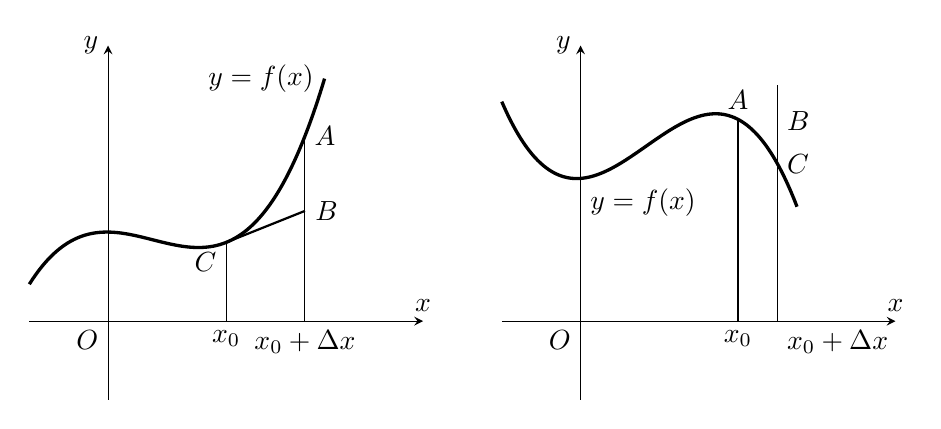
\begin{tikzpicture}[>=stealth]
\begin{scope}
\draw[->](-1,0)--(4,0)node[above]{$x$};
\draw[->](0,-1)--(0,3.5)node[left]{$y$};
\draw[domain=-1:2.75, samples=100, very thick, smooth]plot(\x, {0.25*(\x-.7)*(\x+.5)*(\x-1.5)+1})node[left]{$y=f(x)$};
\node[below left]{$O$};
\draw(1.5,0)node[below]{$x_0$}--(1.5,1)node[below left]{$C$};
\draw(2.5,0)node[below]{$x_0+\Delta x$}--(2.5,2.35)node[right]{$A$};
\draw[thick](2.5,1.4)node[right]{$B$}--(1.5,1);
\end{scope}
\begin{scope}[xshift=6cm]
    \draw[->](-1,0)--(4,0)node[above]{$x$};
\draw[->](0,-1)--(0,3.5)node[left]{$y$};
\draw[domain=-1:2.75, samples=100, very thick, smooth]plot(\x, {-0.3*(\x-.5)*(\x+.5)*(\x-2.5)+2});
\node at (0,1.5)[right]{$y=f(x)$};
\node[below left]{$O$};
\draw(2,0)node[below]{$x_0$}--(2,2.56)node[above]{$A$};
\draw(2.5,0)node[below right]{$x_0+\Delta x$}--(2.5,3);
\node at (2.5,2)[right]{$C$};
\node at (2.5,2.3)[above right]{$B$};
\tkzDefPoints{2.5/2.3/B, 2/2.56/B'}
\tkzDrawLines[add= 1 and 1, thick](B,B')


\end{scope}
\end{tikzpicture}
    \caption*{第3题}
\end{figure}
\item 求下列函数的微分:
\begin{multicols}{2}
    \begin{enumerate}[(1)]
        \item $y=\frac{2}{x^2}$
        \item $y=5\sqrt[3]{x+1}$
        \item $y=(1+2x-x^2)^3$
        \item $y=\cos x^2$
        \item $y=e^x\sin^2 x$
        \item $y=\frac{2x-1}{(x-1)^2}$
        \item $y=\frac{1-x^2}{1+x^2}$
        \item $y=\frac{1}{3}\tan^3\theta+\tan\theta$
    \end{enumerate}
\end{multicols}

\item 计算$\tan 30^{\circ}30'$的近似值(精确到0.0001).
\item 计算$\sin29^{\circ}$的近似值(精确到0.0001).
\item 计算下列各数的近似值(精确到0.0001):
\begin{multicols}{2}
    \begin{enumerate}[(1)]
        \item $\sqrt[5]{1.002}$
        \item $\sqrt[3]{0.998}$
        \item $\ln1.0021$
        \item $\sin0.1^{\circ}$
    \end{enumerate}
\end{multicols}
\end{enumerate}

\begin{center}
    \bfseries B
\end{center}

\begin{enumerate}\setcounter{enumi}{7}
    \item 已知函数$f(x)=x^2$在点$x_0$处自变量$x$的微分$\dd x=0.2$, 对应函数的微分$\dd f(x)=-0.8$,试求$x_0$的值.
    \item   已知函数$y=f[f(x)]$,求$\frac{\dd y}{\dd x}$及$\dd y$.
        \item   已知函数$y=f(\sin x)$,求$\frac{\dd y}{\dd(\sin x)}$及$\frac{\dd y}{\dd x}$.
        \item  单摆的周期$T$(秒)与单摆的长度$\ell$(厘米)之间的函数关系$T=2\pi\sqrt{\frac{\ell}{980}}$,长度为20厘米的单摆加长1厘米后,它的周期大约增加多少?
\end{enumerate}

\section*{四、利用导数研究函数}
过去我们曾研究过函数的性质,现在当我们学习导数后,就可以用导数直接研究函数的性质了,并且方法要比过去简捷.

\section{函数的单调性}
首先我们介绍一个有关导数的十分重要的定理——拉格朗日中值定理.(这个定理的证明留给读者上大学后去完成)

\begin{thm}
    {定理} 如果函数$y=f(x)$在闭区间$[a,b]$上连续,在开区间$(a,b)$内可导,那么在$(a,b)$内至少有一点$\xi$,使得
    \[f'(\xi)=\frac{f(b)-f(a)}{b-a}\]  
\end{thm}

如图12.5,若$[a,b]$上的一段连续曲线,在$(a,b)$内每一点处有切线,则至少有一条切线平行于连结曲线两端点$(a,f(a))$、$(b,f(b))$所成的弦.

\begin{figure}[htp]
    \centering
\begin{tikzpicture}[>=stealth]
    \draw[->](-1,0)--(6,0)node[below]{$x$};
\draw[->](0,-1)--(0,5)node[left]{$y$};
\draw[domain=0:4, smooth, very thick, samples=100]plot(\x+.5, {0.2*(\x-1)*(\x-2)*(\x-3.5)+3.5});
\tkzDefPoints{.5/2.1/A, 4.5/4.1/B}
\node[below left]{$O$};
\draw[dashed](A)node[left]{$A$}--node[right]{$f(a)$}(.5,0)node[below]{$a$};
\draw[dashed](B)node[right]{$B$}--node[right]{$f(b)$}(4.5,0)node[below]{$b$};
\draw(A)--(B);
\tkzDefPoints{1.5/0/C}
\draw[dashed](1.5,0)node[below]{$\xi$}--(1.5,3.5);
\draw[domain=.5:3, thick]plot(\x, {0.5*\x+2.75});



\end{tikzpicture}
    \caption{}
\end{figure}


我们已经学过增函数与减函数的概念,下面学习如何利用导数来判断函数的单调性.

\begin{thm}
    {定理}设函数$f(x)$在闭区间$[a,b]$上连续,在开区间$(a,b)$内可导.
\begin{enumerate}[(1)]
\item 若在$(a,b)$内,$f'(x)>0$,则$f(x)$在$(a,b)$上是增函数;
\item 若在$(a,b)$内,$f'(x)<0$,则$f(x)$在$(a,b)$上是减函数.
\end{enumerate}
\end{thm}

\begin{proof}
设$x_1,x_2\in[a,b]$且 $x_1<x_2$, 则必存在一点 $\xi\; (x_1<\xi<x_2)$, 使得
$$\frac{f(x_{2})-f(x_{1})}{x_{2}-x_{1}}=f'(\xi)$$
即 $f( x_{2}) - f( x_{1}) = f'( \xi ) ( x_{2}- x_{1})$

若 $f'(x)$在$(a,b)$内恒为正,则 $f'({\xi})>0$ 而 $x_2-x_1>0$

$\therefore\quad f( x_{2}) - f( x_{1}) = f'( \xi ) ( x_{2}- x_{1}) > 0$ 即
$f(x_{2})>f(x_{1})$. 得出 $f(x)$在$(a,b)$上是增函数。

若$f'(x)$在$(a,b)$内恒为负,则 $f'(\xi)<0$, 而 $x_{2}-x_{1}>0$

$\therefore\quad f( x_{2}) - f( x_{1}) = f'( \xi ) ( x_{2}- x_{1}) < 0$即$f(x_{2})<f(x_1)$. 得出$f(x)$在$(a,b)$上是减函数.

另外,若在开区间$(a,b)$内 $f'(x)\equiv 0$,则 $f'({\xi})\equiv0,\; (x_{1}<\xi<x_{2})$, 因此有 $f(x_{2})\equiv f(x_{1})$, 这样 $f(x)$在区间$[a,b]$上是常数.
\end{proof}



\begin{example}
    求函数$f(x)=x^3-x^2-x+5$的单调区间
\end{example}

\begin{solution}
$f(x)=x^3-x^2-x+5,\qquad f'\left(x\right)=3x^{2}-2x-1=\left(3x+1\right)\left(x-1\right)$

$\because\quad $ 当 $x<-\frac13$或 $x>1$ 时,$f'(x)>0$.

$\therefore\quad f( x)$的递增区间是$\left(-\infty,\; -\frac13\right)$和$(1,+\infty)$.

$\because\quad $ 当$-\frac13<x<1$时,$f'(x)<0$. 

$\therefore\quad f( x)$的递减区间是$\left(-\frac13,\; 1\right).$
\end{solution}

\begin{example}
    求函数$f(x)=(x-2)^2(x+1)^3$的单调区间
\end{example}

\begin{solution}
\[\begin{split}
    f(x)&=(x-2)^2(x+1)^3\\
f'(x)&=2(x-2)(x+1)^{3}+3(x-2)^{2}(x+1)^{2}=(x-2)(x+1)^{2}(5x-4)
\end{split}\]
令$f'( x) = 0$ 得 $x= - 1,\; \frac 54,\; 2$.
\begin{center}
    \begin{tabular}{c|cccc}
\hline
& $(-\infty,-1)$ & $\left(-1,\frac{5}{4}\right)$ & $\left(\frac{5}{4},2\right)$ & $(2,+\infty)$ \\ 
\hline
$f'(x)$&  $+$&  $+$&  $-$&  $+$\\
$f(x)$ & $\nearrow$& $\nearrow$& $\searrow$& $\nearrow$\\
\hline
    \end{tabular}
\end{center}

$f(x)$的递增区间是$\left(-\infty,\; \frac{5}{4}\right)$, $(2,+\infty)$;递减区间是
$\left(\frac{5}{4},\; 2\right).$
\end{solution}

\begin{example}
    求证:若 $x\in\left(0,\; \frac\pi2\right)$, 则 $\tan x>\sin x$.
\end{example}

\begin{analyze}
    欲证$\tan x>\sin x$, 只需证$\tan x-\sin x>0$, 若设 $f(x) =\tan x-\sin x$,
    
$\because\quad  f(0)=0$, 只需证当 $x\in\left(0,\; \frac\pi2\right)$时,$f(x)>f(0)$.
\end{analyze}

\begin{proof}
    设$f(x)=\tan x- \sin x\quad x\in \left [ 0,\; \frac \pi 2\right )$

$\because\quad f'( x) = \sec ^{2}x- \cos x= \frac {1- \cos ^{3}x}{\cos ^{2}x}> 0$, 
其中$x\in\left(0,\; \frac\pi2\right)$.

$\therefore\quad f( x) =\tan x-\sin x$ 在区间$\left[0,\; \frac\pi2\right)$是增函数

即当$0<x<\frac{\pi}{2}$时,$f(x)>f(0)=0$. 

$\therefore\quad \tan x>\sin x$, 其中$x\in\left(0,\frac\pi2\right)$.
\end{proof}

\begin{ex}
\begin{enumerate}
    \item 求下列函数的单调区间:
\begin{multicols}{2}
\begin{enumerate}[(1)]
    \item $y=\frac{2x}{1+x^2}$
\item $y=x-e^{x}$
\item $y= \ln ( x+ \sqrt {1+ x^{2}})$ 
\item $y=(x-1)(x+1)^{3}$
\end{enumerate}
\end{multicols}

    
\item    证明不等式:
\begin{enumerate}[(1)]
    \item $\frac{1}{3}(x-1)>\sqrt[3]{x}-1$, 其中$x\in ( 1, + \infty )$
    \item $\ln(1+x)>x-\frac{1}{2}x^{2}$, 其中 $x\in(0,+\infty)$
\end{enumerate}
\end{enumerate} 
\end{ex}

\section{函数的极大值与极小值}
请看图12.6至图12.9:

\noindent
\begin{minipage}{.48\textwidth}
    \centering
\begin{tikzpicture}[>=stealth]
    \draw[->](-1,0)--(5,0)node[below]{$x$};
    \draw[->](0,-1)--(0,4)node[left]{$y$};
\node[below left]{$O$};
\draw[very thick](2,1)node[right]{极小} arc (0:90:2.2);
\draw[very thick](2,1) arc (180:90:2)node[above]{$y=f(x)$};
\draw[dashed](2,1)--(2,0)node[below]{$x_0$};
\node at (2,0){\small (\quad)};
\end{tikzpicture}    
\captionof{figure}{}
\end{minipage}\hfill
\begin{minipage}{.48\textwidth}
        \centering
\begin{tikzpicture}[>=stealth]
    \draw[->](-1,0)--(5,0)node[below]{$x$};
    \draw[->](0,-1)--(0,4)node[left]{$y$};
    \node[below left]{$O$};
\draw[domain=pi/2:pi*1.5, smooth, samples=100, very thick]plot(\x-.5, {sin(2*\x r)+2.5})node[below ]{$y=f(x)$};
\draw[dashed](.75*pi-.5,0)node[below]{$x_0$}--(.75*pi-.5, 1.5);
\node at (.75*pi-.5,0){\small (\quad)};
\draw[thick](.75*pi-1, 1.5)--(.75*pi, 1.5)node[right]{极小};
\end{tikzpicture}    
\captionof{figure}{}
\end{minipage}

\noindent
\begin{minipage}{.48\textwidth}
    \centering
\begin{tikzpicture}[>=stealth]
    \draw[->](-1,0)--(5,0)node[below]{$x$};
    \draw[->](0,-1)--(0,4)node[left]{$y$};
\node[below left]{$O$};
\draw[domain=.25:2.85, smooth, samples=100, very thick]plot(\x+.5, {.6*(\x-.8)*(\x-1.5)*(\x-2.5)+2})node[above]{$y=f(x)$};
\draw[dashed](1.6,2.12)--(1.6,0)node[below]{$x_0$};
\node at (1.6,0){\small (\quad)};
\draw[thick](1.6-.5,2.12)--node[above]{极大}(1.6+.5,2.12);

\end{tikzpicture}    
\captionof{figure}{}
\end{minipage}\hfill
\begin{minipage}{.48\textwidth}
        \centering
\begin{tikzpicture}[>=stealth]
    \draw[->](-1,0)--(5,0)node[below]{$x$};
    \draw[->](0,-1)--(0,4)node[left]{$y$};
    \node[below left]{$O$};
\draw[very thick](.25,1)--(1.8,3);
\draw[very thick](1.8,3)arc (-170:-20:1.5);
\node at (1.8,0){\small (\quad)};
\draw[dashed](1.8,0)node[below]{$x_0$}--(1.8,3)node[above]{极大};
\node at (3.7,2.5){$y=f(x)$};
\end{tikzpicture}    
\captionof{figure}{}
\end{minipage}

在图12.6和图12.7中,$f(x_0)$的值小于点$x_0$的附近中的
其它函数值;在图12.8和图12.9中,$f(x_0)$的值大于点$x_0$的附近中的其它函数值.

\begin{thm}
{定义} 设函数$y=f(x)$在点$x_0$处连续,并且$x_0$不是其定义区间的端点,$x$是点$x_0$的附近$(x_0-\delta,x_0+\delta)$中异于$x_0$的任意一点.
\begin{enumerate}[(1)]
\item 若恒有$f(x)>f(x_0)$,则称函数$f(x)$在点$x_0$处有一极小值$f(x_0)$, $x_0$称为函数$f(x)$的一个极小值点.
\item 若恒有$f(x)<f(x_0)$,则称函数$f(x)$在点$x_0$处有一极小值$f(x_0)$, $x_0$称为函数$f(x)$的一个极大值点.
\end{enumerate}
函数的极大值和极小值可统称为函数的极值.
\end{thm}


从图12.7和图12.8可看出,若$f(x)$在点$x_0$处有极值,且$f(x)$在点$x_0$可导,则函数$y=f(x)$的图象在点$(x_0,f(x_0))$处的切线平行于$x$轴. 即$f'(x_0)=0$.(证明从略).

若$f(x)$可导,把$f'(x)=0$的解称为函数$f(x)$的驻点.

显然,可导函数的极值点一定是驻点. 由于函数$y=x^3$的驻点$x=0$既不是函数$y=x^3$的极大值点,也不是其极小值点,所以,可导函数的驻点不一定是函数的极值点.


\noindent
\begin{minipage}{.48\textwidth}
    \centering
\begin{tikzpicture}[>=stealth]
    \draw[->](-1,0)--(4,0)node[below]{$x$};
    \draw[->](0,-1)--(0,4)node[left]{$y$};
\node[below left]{$O$};

\draw[domain=-1.5:1.5, smooth, samples=100, very thick]plot(\x+2, {-.5*\x*\x+2.5});
\draw[dashed](2,2.5)--(2,0)node[below]{$x_0$};
\node at (2,0){\small (\quad)};
\node at (2,-.75){(极大值点)};
\draw[thick](2+1,2.5)--node[above]{$f'(x_0)=0$}(2-1,2.5);
\node at (1,2)[left]{$f'(x)>0$};
\node at (3,2)[right]{$f'(x)<0$};

\draw[->](1,1.5)--+(.5,.5);
\draw[->](2.5,2)--+(.5,-.5);

\end{tikzpicture}    
\captionof{figure}{}
\end{minipage}\hfill
\begin{minipage}{.48\textwidth}
        \centering
\begin{tikzpicture}[>=stealth]
    \draw[->](-1,0)--(5,0)node[below]{$x$};
    \draw[->](0,-1)--(0,4)node[left]{$y$};
\node[below left]{$O$};

\draw[domain=-1.5:1.5, smooth, samples=100, very thick]plot(\x+2, {.5*\x*\x+2});

\draw[dashed](2,2)--(2,0)node[below]{$x_0$};
\node at (2,0){\small (\quad)};

\node at (2,0){\small (\quad)};
\node at (2,-.75){(极小值点)};


\draw[thick](2+1,2)--node[below, fill=white]{$f'(x_0)=0$}(2-1,2);
\node at (1,2.5)[left]{$f'(x)<0$};
\node at (3,2.5)[right]{$f'(x)>0$};

\draw[->](1,2.85)--+(.5,-.5);
\draw[->](2.5,2.35)--+(.5,.5);


\end{tikzpicture}    
\captionof{figure}{}
\end{minipage}

由图12.10 可知,对于可导函数$y=f(x)$, $f'(x_0)=0$, 若当 $x\in(x_0-\delta,x_0)$时,$f'(x)>0$;当 $x\in(x_0,x_0+\delta)$时,$f'(x)<0$, 则函数 $f(x)$在点 $x_0$ 处有极大值 $f(x_0)$.

由图 12.11 可知,对于可导函数 $y=f(x)$, $f'(x_0)=0$, 若当$x\in(x_{0}-\delta,x_{0})$时,$f'(x)<0$;当$x\in(x_{0},x_{0}+\delta)$时,$f'(x)>0$, 则函数 $f(x)$在点 $x_0$ 处有极小值 $f(x_0)$.

为此,我们给出求可导函数 $y=f(x)$的极值的一种方法:
\begin{enumerate}
\item 求 $f(x)$的导数 $f'(x)$;
\item 求$f(x)$在定义域内的驻点即求方程 $f'(x)=0$ 的根;
\item 考查$f'(x)$在驻点$x_{0}$左右的符号:
\begin{enumerate}[(1)]
    \item 若“左正右负”, 则$f(x)$在点$x_0$处有极大值$f(x_0)$; 
    \item 若“左负右正”, 则$f(x)$在点$x_0$处有极小值$f(x_0)$;
    \item 若“左右同号”, 则 $f(x)$在点 $x_0$ 处无极值.
\end{enumerate}
\end{enumerate}

\begin{example}
求函数$f(x)=\frac{1}{3}x^{3}-4x+4$的极值.
\end{example}

\begin{solution}
$f(x)=\frac{1}{3}x^{3}-4x+4\quad f'(x)=x^{2}-4=(x-2)(x+2)$

令$f'(x)=0$, 得$x_{1}=2,\quad x_{2}=-2$.
\begin{center}
    \begin{tabular}{c|ccccc}
\hline
$x$&$(-\infty,-2)$& $-2$& $(-2,2)$& 2&$(2,+\infty)$\\
\hline
$f'(x)$ &  $+$  &  0  & $-$   &  0  & $+$ \\ 
$f(x)$ &  $\nearrow$  &  极大值  &  $\searrow$  &  极小值  &  $\nearrow$\\ 
\hline
    \end{tabular}
\end{center}
\[\begin{split}
    \therefore\quad  y_{\text{极大}}&=f(-2)=\frac{1}{3}\x (-2)^3-4\x(-2)+4=9\frac{1}{3}\\
    y_{\text{极小}}&=f(2)=\frac{1}{3}\x 2^3-4\x 2+4=-1\frac{1}{3}\\
\end{split}\]
\end{solution}

\begin{example}
    求函数$f(x)=x^3-3x^2+3x+2$的极值.
\end{example}

\begin{solution}
    $f(x)=x^3-3x^2+3x+2$

$\because\quad f'(x)=3x^2-6x+3=3(x-1)^2\ge 0$

$\therefore\quad x=1$虽是$f(x)$的驻点,但不是$f(x)$的极值点

$\therefore\quad $函数$f(x)=x^3-3x^2+3x+2$无极值.
\end{solution}



\begin{example}
    求函数$f(x)=-x^{\tfrac{2}{3}}$的极值.
\end{example}

\begin{solution}
    $f(x)=-x^{\tfrac{2}{3}}$

$\because\quad    f'(x)=-\frac{2}{3\sqrt[3]{x}}\ne 0\quad (x\ne 0)$

$\therefore\quad f(x)$在点$x=0$处不可导,当$x\ne 0$时,$f(x)$无驻点.

又$\because\quad f(x)$在点$x=0$处连续. 当$x<0$时,$f'(x)>0$;$x>0$时,$f'(x)<0$.

$\therefore\quad $当$x=0$时,$f(x)$有极大值0.
\end{solution}

\begin{rmk}
    在用求导的方法求$f(x)$的极值时,对于不可导点,要考查$f(x)$在该点附近的单调性及在这个点的连续性,以确定此点是否为$f(x)$的极值点.
\end{rmk}


\begin{ex}
\begin{enumerate}
    \item 求下列函数的极值:
\begin{multicols}{2}
\begin{enumerate}[(1)]
\item $y=2x^3-6x^2-18x+7$
\item $y=x-\ln(1+x)$
\item $y=x+\sqrt{1-x}$
\item $y=\frac{3x^2+4x+4}{x^2+x+1}$
\end{enumerate}
\end{multicols}

    \item 求函数$y=x^x\; (x\ge 0.1)$的极值.
\end{enumerate}
\end{ex}

\section{函数的最大值与最小值}
我们知道,函数的最大值与最小值又可统称为函数的最值,求最值的问题在实际中是很多的,例如,在一定条件下使“用料最省”、“容积最大”、“功率最大”、“运费最少”等.本节所学的最值问题,是在求函数极值(即函数在一个点的邻域内的最值)的基础上,研究函数在给定区间上的最值问题.

在12.4节中介绍连续函数的性质时,我们曾指出,定义在闭区间$[a,b]$上的连续函数一定有最大值和最小值. 我们学了函数的极值后,只要求出函数$f(x)$在区间$[a,b]$内的一切极值和函数在区间端点的值$f(a)$及$f(b)$,其中最大者就是函数的最大值,而其中最小者即为函数的最小值(如图12.12).

\begin{figure}[htp]
    \centering
\begin{tikzpicture}[>=stealth]
    





\end{tikzpicture}
    \caption{}
\end{figure}


\begin{example}
求函数$f(x)=x^3-3x^2-9x+2$在区间$[-2,5]$上的最大值和最小值.
\end{example}

\begin{analyze}
    确定函数的最大、最小值的关键是比较函数的极值和区间端点$f(x)$的值的大小.
\end{analyze}

\begin{solution}
$f(x)=x^3-3x^2-9x+2,\qquad 
f'(x)=3x^2-6x-9=3(x^2-2x-3)$

令$f'(x)=0$,即$x^2-2x-3=0$

解这个二次方程,得$f(x)$的驻点为
$x_1=-1,\quad x_2=3$

\[\begin{split}
    \because\quad f(-1)&=-1-3+9+2=7\qquad \text{($x=-1$是极大值点)}\\
f(3)&=27-27-27+2=-25\qquad  \text{($x=3$是极小值点)}\\
f(-2)&=-8-12+18+2=0\\
f(5)&=125-75-45+2=7
\end{split}\]

$\therefore\quad $在区间$[-2,5]$上函数$f(x)$的最大值为7,最小值为$-25$.
\end{solution}

\begin{example}
    在测量某物理量的过程中,因仪器和观察的误差, 使得$n$次 测 量 分 别 得 到$x_1, x_2, x_3, x_4,\ldots , x_n$共$n$个数据,试求量$x$, 使得它与这$n$个值的差的平方和最小。
\end{example}

\begin{solution}
按题意,设
\[\begin{split}
    f(x)&=(x-x_{1})^{2}+(x-x_{2})^{2}+\cdots+(x-x_{n})^{2}\\
   f'(x)&=2(x-x_{1})+2(x-x_{2})+\cdots+2(x-x_{n})=2[nx-(x_{1}+x_{2}+\cdots+x_{n})]
\end{split}\]

令 $f'(x)=0$, 解得 $f(x)$的一个驻点为
$x=\frac{x_{1}+x_{2}+\cdots+x_{n}}{n}$

又$\because\quad$ 当$x< \frac {x_{1}+ x_{2}+ \cdots + x_{n}}n$时,$f'(x)<0$;当
$x>\frac{x_1+x_2+\cdots+x_n}n$时,$f'(x)>0$

$\therefore\quad x= \frac {x_{1}+ x_{2}+ \cdots + x_{n}}n$既为 $f(x)$极小值点又为 $f(x)$
的 最 小 值 点 . 故  $x= \frac {x_{1}+ x_{2}+ \cdots + x_{n}}n$为所求.
  \end{solution}

\begin{rmk}
    若由问题的实际情况可以断定:可导函数 $f(x)$在定义域开区间内存在最大值(或最小值),而且$f(x)$在此区间内的\textbf{驻点唯一},那么可立即断定这个驻点所对应的函数值为$f(x)$的最大值(或最小值). 这一点在解决某些实际问题时很有用.
\end{rmk}

\begin{example}
已 知 : 直 线 $y= 2x+ m\; ( m> 0)$ 与 抛 物 线 $y= - \frac 12x^{2} +6$ 交于 $A,B$ 两点, $P(2,4)$是抛物线上一定点,试求$\triangle PAB$面积的最大值.
\end{example}

\begin{solution}
$\begin{cases}
    y=2x+m& m>0\\
    y=-\frac{1}{2}x^{2}+6
\end{cases}$ 
消去$y$得
$$x^2+4x+2(m-6)=0$$

\[\begin{cases}
    \Delta =16-8(m-6)=8(8-m)>0\\
    m>0
\end{cases}\]
得  $0<m<8$

又$\because\quad | AB| = \sqrt {5}\left | x_{A}- x_{B}\right |=2\sqrt{10}\sqrt{8-m}$

$P$点到直线 $AB$ 的距离
$$d=\frac{|4-4+m|}{\sqrt{5}}=\frac{m}{\sqrt{5}}$$

$\therefore\quad \triangle PAB$的面积$S$ 为
$$S=\frac{1}{2}\cdot\frac{m}{\sqrt{5}}\cdot2\sqrt{10}\sqrt{8-m}=\sqrt{2(8m^{2}-m^{3})}$$
其中$0<m<8$

$$S^{\prime}=\frac{2(16m-3m^{2})}{2\sqrt{2(8m^{2}-m^{3})}}=\frac{m(16-3m)}{\sqrt{2(8m^{2}-m^{3})}}$$

    令$S'=0$,得$m=\frac{16}{3}$.

$\because\quad $在区间$(0,8)$内函数有唯一驻点$m=\frac{16}{3}$. 且$\triangle PAB$的面积$S$有最大值.

$\therefore\quad $当$m=\frac{16}{3}$时,$S_{\triangle ABC}$有最大值
\[S_{\max}= \frac{16}{3}\x \sqrt{2}\x\sqrt{8-\frac{16}{3}}=\frac{64\sqrt{3}}{9} \]
\end{solution}

\begin{example}
    从南到北的铁路干线经过甲、乙两城,两城之间的距离为150千米,某工厂位于乙城正西60千米,现要从甲城把货物运往工厂,在铁路上的运费为每千米4元,而沿公路上的运费为每千米6元,为了使货物从甲城运到工厂的运费最省,应该从铁路干线上的何处起修筑一条通往工厂的公路较为适宜?
\end{example}

\begin{solution}

\noindent
\begin{minipage}{.6\textwidth}
 \CTEXindent   如图12.13,设从铁路干线$S$处修一条通往工厂$F$处的公路($S$距乙城$x$千米),货物运费为$W$元,则
\[W=4(150-x)+6\sqrt{x^2+3600}\]
其中$0<x<150$
\[\begin{split}
    W'&=-4+\frac{6x}{\sqrt{x^2+3600}}\\
    &=\frac{6x-4\sqrt{x^2+3600}}{\sqrt{x^2+3600}}
\end{split}\]
\end{minipage}
\hfill
\begin{minipage}{.35\textwidth}
\centering
\begin{tikzpicture}[scale=.8]
\tkzDefPoints{0/0/A, 0/-5/B, 0/-2/S, -2.5/0/F}
\draw(B)node[right]{甲}--(A)node[right]{乙}--node[above]{$60$}(F)node[left]{$F$}--(S)node[right]{$S$};
\tkzMarkRightAngles[size=.2](B,A,F)
\node at  (0,-1)[right]{$x$};
\end{tikzpicture}
\captionof{figure}{}
\end{minipage}

令$W'=0$,则
\[\begin{split}
    3x&=2\sqrt{x^2+3600}\\
    5x^2&=4\x 3600\\
    x^2&=24^2\x 5
\end{split}\]

$\therefore\quad x=24\sqrt{5}\approx 53.666.$

$\because\quad $驻点唯一,且此问题有最小值.

$\therefore\quad x=24\sqrt{5}\approx 53.666$为运费函数的最小值点.    

答:可在铁路干线上,距乙城约53.666千米处修一条到工厂的公路,使运费最省.
\end{solution}

\begin{ex}
\begin{enumerate}
    \item 在本节(12.15节)中,例12.31、例12.32、例12.33的初等解法是什么?
    \item 用边长为60cm的正方形铁皮做一个无盖水箱,先在四角分别截去一个小正方形,然后把四边翻转$90^{\circ}$,再焊接而成. 问水箱底边的长应取多少,才能使水箱容积最大,最大容积是多少?
    \item 求函数$y=-3x^4+6x^2-1\; (-2\le x\le 2)$的最大值和最小值.
\end{enumerate}
\end{ex}

\section{函数的图象的凸性与拐点}

我们过去在作函数的图象时曾经遇到这样一个问题,同
是给定区间上的增(或减)函数,但函数的图象的几何性态却
不同,例如图 12.14 中的图象,曲线上升有四种情况:

一般地设函数 $y=f(x)$定义在区间$[a,b]$上,若对于任意
$x_{1},x_{2}\in[a,b]$且$x_1<x_{2}$,
\begin{enumerate}
    \item 若总有$f\left(\frac{x_{1}+x_{2}}{2}\right)>\frac{f(x_{1})+f(x_{2})}{2}$,
则称函数 $y=f(x)$的图象在区间$[a,b]$上凸;
\item 若总有$f\left(\frac{x_{1}+x_{2}}{2}\right)<\frac{f(x_{1})+f(x_{2})}{2}$,则称函数$y=
f(x)$的图象在区间$[a,b]$下凸(如图 12.15).
\end{enumerate}

\begin{figure}[htp]
    \centering
\begin{tikzpicture}[>=stealth]
\begin{scope}
\draw[->](-1,0)--(4,0)node[below]{$x$};
\draw[->](0,-1)--(0,4)node[left]{$y$};
\node[below left]{$O$};
\draw[domain=0:2, smooth, samples=100, very thick]plot(\x, {\x*\x})node[below right, text width=2cm, align=center]{$y=x^2$\\$(x>0)$};
\node at (2,-.75){(1)};

\end{scope}
\begin{scope}[xshift=6cm]
    \draw[->](-1,0)--(4,0)node[below]{$x$};
\draw[->](0,-1)--(0,4)node[left]{$y$};
\node[below left]{$O$};
\draw[domain=0:2, smooth, samples=100, very thick]plot({\x*\x},\x)node[above left]{$y=\sqrt{x}$};
\node at (2,-.75){(2)};
\end{scope}
\begin{scope}[yshift=-4cm, xshift=1.5cm]
    \draw[->](-2.5,0)--(2.5,0)node[below]{$x$};
    \draw[->](0,-2)node[below]{(3)}--(0,2)node[left]{$y$};
    \node[below right]{$O$};
\draw[domain=-pi/2:pi/2, smooth, very thick, samples=100]plot(\x, {sin(\x r)});
\foreach \x in {-pi/2, pi/2}
{
    \draw[dashed](\x,0)--(\x,\x*2/pi);
}
\node at (1.5,-1)[text width=3cm, align=center]{$y=\sin x$\\$\left(-\frac{\pi}{2}\le x\le \frac{\pi}{2}\right)$};
\end{scope}
\begin{scope}[yshift=-4cm, xshift=7.5cm]
    \draw[->](-2.5,0)--(2.5,0)node[below]{$x$};
    \draw[->](0,-2)node[below]{(4)}--(0,2)node[left]{$y$};
    \node[below right]{$O$};
    \draw[domain=-1.2:1.2, smooth, very thick, samples=100]plot(\x, {\x^3})node[below right]{$y=x^3$};
\end{scope}    
\end{tikzpicture}
    \caption{}
\end{figure}











\begin{example}
    
\end{example}

\begin{solution}
    
\end{solution}



\begin{example}
    
\end{example}

\begin{solution}
    
\end{solution}



\begin{example}
    
\end{example}

\begin{solution}
    
\end{solution}



\begin{example}
    
\end{example}

\begin{solution}
    
\end{solution}



\begin{example}
    
\end{example}

\begin{solution}
    
\end{solution}



\begin{example}
    
\end{example}

\begin{solution}
    
\end{solution}






\begin{thm}
{定理} 设函数$y=f(x)$在开区间$(a,b)$内有二阶导数.
\begin{enumerate}[(1)]
\item 若对于任意的$x\in (a,b)$, $f''(x)>0$,则曲线$y=f(x)$在区间$(a,b)$内下凸;
\item 若对于任意的$x\in (a,b)$, $f''(x)<0$,则曲线$y=f(x)$在区间$(a,b)$内上凸.  
\end{enumerate}
\end{thm}

此定理只作如前的说明,它的证明留给读者上大学后完成.

\begin{example}
    求证:正弦曲线$y=\sin x$在$(0,\pi)$上是上凸.
\end{example}

\begin{proof}
\[y=\sin x,\quad y'=\cos x,\quad y''=-\sin x\]

$\because\quad $当$x\in(0,\pi)$时,$y''=-sinx<0$

$\therefore\quad $正弦曲线$y=\sin x$在区间$(0,\pi)$是上凸的.
\end{proof}

大家知道,对于函数$f(x)=\sin x\; (x\in (0,\pi))$, $x=\frac{\pi}{2}$是它的极大值点,$f'(x)$在点$\frac{\pi}{2}$附近的符号是“左正右负”与函数的图象上凸是一致的,因此,又可用$f''(x)$在该点值的正负来判定驻点是函数的极大值点还是极小值点. 下面给出一种利用二阶导数来判定函数极值的方法(证明留给读者).

\begin{thm}
    {定理} 设$f(x_0)=0$且$f''(x_0)$存在
\begin{enumerate}[(1)]
\item 若$f''(x_0)>0$,则$f(x)$在点$x_0$处有极小值$f(x_0)$;
\item 若$f''(x_0)<0$,则$f(x)$在点$x_0$处有极大值$f(x_0)$.
\end{enumerate}
\end{thm}


\begin{example}
    求函数$f(x)=\frac{1}{3}x^3-4x+4$的极值.
\end{example}

\begin{solution}
\[\begin{split}
    f(x)&=\frac{1}{3}x^3-4x+4\\
f'(x)&=x^2-4=(x-2)(x+2)\\
f''(x)&=2x
\end{split}\]
令$f'(x)=0$,解得$f(x)$的驻点为$x_1=2$、$x_2=-2$

$\because\quad f''(2)=4>0$

$\therefore\quad y_{\text{极小}}=f(2)=\frac{8}{3}-8+4=-\frac{4}{3}$

$\because\quad f''(-2)=-4<0$

$\therefore\quad y_{\text{极大}}=f(-2)=-\frac{8}{3}+8+4=\frac{28}{3}$.

对于函数$y=x^3$, 点$x=0$是曲线$y=x^3$由左半部分上凸转为右半部分下凸的分界点,并且$f'(0)=0$, $f''(0)=0$,像这样的点我们称它为曲线的拐点.
\end{solution}

\begin{thm}
    {定义} 设函数$y=f(x)$的图象上一点$P(x_0,f(x_0))$恰为曲线$y=f(x)$上凸与下凸部分的分界点,则称点$P(x_0, f(x_0))$为曲线$y=f(x)$的拐点,$x_0$称为函数$f(x)$的拐点.
\end{thm}



\begin{example}
    求函数$f(x)=\sin x$的拐点.
\end{example}

\begin{solution}
    \[f(x)=\sin x,\quad f'(x)=\cos x,\quad f''(x)=-\sin x\]
令$f''(x)=0$得$x=k\pi\; (k\in\Z)$

又$\because\quad f''(x)$在点$k\pi$的两侧异号

$\therefore\quad x=k\pi\; (k\in\Z)$为$f(x)=\sin x$的拐点.
\end{solution}

一般地,设函数$f(x)$在点$x_0$处的附近有二阶导数,并且:
\begin{enumerate}[(1)]
\item $f''(x_0)=0$;
\item $f''(x)$的值在点的两侧异号
\end{enumerate}
则点$P(x_0,f(x_0))$为函数$y=f(x)$图象的拐点.

类似于$f'(x_0)=0$是点$x_0$为$f(x)$的极值点的必要条件一样, $f''(x)=0$是点$x_0$为$f(x)$的拐点的必要条件,而不是充分条件. 例如,$f(x)=x^6$, $f''(x)=30x^4$,当$x\ne 0$时,$f''(x)>0$,故曲线$y=x^6$下凸,虽然$f''(0)=0$,但$x=0$不是函数的拐点,而是极小值点.

\begin{ex}
\begin{enumerate}
    \item 求曲线$y=\arctan x$的上凸、下凸区间及拐点.
    \item 求证函数$y=a^x$ ($a>0$且$a\ne 1$)的图象下凸.
    \item 求$f(x)=x^3-3x^2-9x+14$的极值及拐点.
\end{enumerate}
\end{ex}

\section{函数的图象绘制}
前面我们对函数的性质进行了进一步的研究,这就使我们能依据函数的性质,更准确地作出函数的图象. 今后在绘制
一个函数的图象之前,一般应依次对函数作如下分析,然后列表画图.
\begin{enumerate}
\item 确定函数的定义域和值域(可大致确定图象的范围);
\item 验证函数的奇偶性、周期性(可缩小研究函数的范围);
\item 找出函数图象的某些特殊点(例如图象与坐标轴的交点、间断点及其他特殊点);
\item 利用导数求出函数的单调区间、极值点和极值、图象的上凸或下凸区间、拐点等;
\item 考察函数的图象是否有渐近线(了解图象若无限延伸时,它的变化趋势).
\end{enumerate}





\begin{example}
    试作函数 $f(x)=\frac{x^{2}}{x+1}$的图象
\end{example}

\begin{solution}
    对于函数$f(x)=\frac{x^2}{x+1}$,
\begin{enumerate}[(1)]
    \item $x\in ( - \infty , - 1) \cup ( - 1, + \infty )$ 
    \item 当$x\in(-\infty,-1)$时,$f(x)<0$;当$x\in(-1,+\infty)$时$f(x)\geqslant0$;(当且仅当 $x=0$ 时,$f(x)=0$)
    \item $f'(x)=\frac{x^2+2x}{(x+1)^2}$

令 $f'\left(x\right)=0$, 解得驻点 $x_1=0,\quad x=-2$.
$$f''(x)=\frac{2(x+1)(x+1)^2-2(x+1)(x^2+2x)}{(x+1)^4}=\frac{2}{(x+1)^{3}}$$

$\because\quad f''( 0) > 0$

$\therefore\quad y_{\text{极 小 }}= f( 0) = 0$.

又$\because\quad f'' (-2)<0$

$\therefore\quad  y_{\text{极大}}=f(-2)=-4$.

\item $\because\quad$当$x\in ( - \infty , - 1)$时, $f''( x) < 0$,

$\therefore\quad $ 函数 $f(x)$的图象在区间$(-\infty,-1)$内上凸

$\because\quad $ 当$x\in(-1,+\infty)$时, $f''(x)>0$

$\therefore\quad$ 函数 $f(x)$的图象在区间$(-1,-\infty)$内下凸

\item $f(x)$的递增区间是$(-\infty,-2]$, $[0,+\infty)$; 递减区间
是$[-2,-1)$, $(-1,0]$

\item $\because\quad f( x) = \frac {x^{2}}{x+ 1}= \frac {( x^{2}- 1) + 1}{x+ 1}=(x-1)+\frac{1}{x+1}$

当 $x\to\infty$时,$f(x)\approx x-1$ 且 $f(x)\to\infty$

$\therefore\quad $ 当  $x\to \infty$时,曲线 $y=f(x)$上的点到直线 $y=x-1$
的距离$d\to0$.

又$\because\quad \Lim{x}{- 1^{+}}f( x) = + \infty,\quad \Lim{x}{- 1^{- }}f( x) = - \infty$,

$\therefore\quad $ 函数 $f(x)$的图象的渐近线方程是 $x=-1$ 和
$y=x-1$.

\item 由 以 上 分 析$f( x) \in ( - \infty , - 4) \cup [ 0, + \infty ) $.
\end{enumerate}
上述要点可汇总如下表:
\begin{center}\small
\begin{tabular}{cccccccc}
    \hline
$x$ & $(-\infty,-2)$ & $-2$ & $(-2,-1)$ & $-1$ & $(-1,0)$ & $0$ & $(0,+\infty)$\\
\hline
$f'(x)$   &    $+$     &  0       & $-$        &         & $-$        &   0      & $+$\\        
$f''(x)$   &   $-$      &     $-$    &    $-$     &         &      $+$   &   $+$      & $+$\\     
$f(x)$   & $-\infty\nearrow-4$& $-4$& $-4\searrow -\infty$&间断点&$+\infty\searrow 0$& 0& $0\nearrow +\infty$\\
&   &    极大值     &         &         &       &   极小值      &   \\
\hline
\end{tabular}
\end{center}
函数$f(x)=\frac{x^2}{x+1}$的图象如图12.17.
\begin{figure}[htp]
    \centering
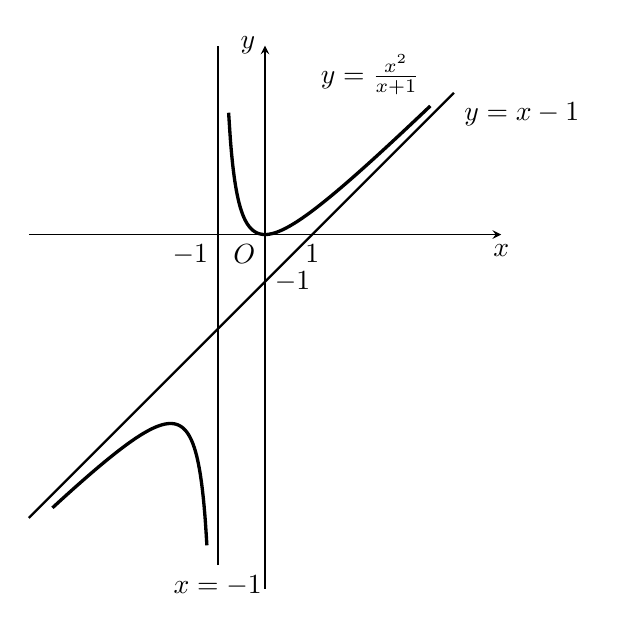
\begin{tikzpicture}[>=stealth, scale=.6]
\draw[->](-5,0)--(5,0)node[below]{$x$};
\draw[->](0,-7.5)--(0,4)node[left]{$y$};
\draw[domain=-5:4, thick, smooth]plot(\x, \x-1)node[below right]{$y=x-1$};
\draw[thick](-1,-7)node[below]{$x=-1$}--(-1,4);
\draw[domain=-1+.23:3.5, smooth, very thick, samples=100]plot(\x, {\x-1+1/(\x+1)})node[above left]{$y=\frac{x^2}{x+1}$};
\draw[domain=-1-.23:-4.5, smooth, very thick, samples=100]plot(\x, {\x-1+1/(\x+1)});
\node [below left]{$O$};
\node at (0,-1)[right]{$-1$};
\node at (-1,0)[below left]{$-1$};
\node at (1,0)[below]{$1$};
\end{tikzpicture}
    \caption{}
\end{figure}

\begin{center}
\begin{tabular}{c|ccccc}
\hline
$x$ & $-3$ & $-\frac{3}{2}$ & $-\frac{1}{2}$  &  1 &2  \\[1.5ex]
\hline
$y$ & $-\frac{9}{2}$&$-\frac{9}{2}$&$\frac{1}{2}$&$\frac{1}{2}$&$\frac{4}{3}$\\[1.5ex]
\hline
\end{tabular}
\end{center}

\end{solution}

\begin{ex}
作下列函数的图象:
\begin{multicols}{2}
\begin{enumerate}
    \item $y=\frac{x}{x^2+1}$
    \item $y=x-\ln(x+1)$
\end{enumerate}
\end{multicols}
\end{ex}



\section*{习题五}
\begin{center}
    \bfseries A
\end{center}

\begin{enumerate}
    \item 求下列函数的单调区间:
\begin{multicols}{2}
\begin{enumerate}[(1)]
 \item $y=x^3-6x^2+9x-3$
\item $y= \sqrt [ 3] {x^2+ 1}$ 
\item $y=\frac{x}{x^{2}+1}$
\item $y=x-2\sin x\quad (0\leqslant x\leqslant 2\pi)$   
\end{enumerate}
\end{multicols}

\item    求下列函数的极值:
\begin{multicols}{2}
\begin{enumerate}[(1)]
\item $y=\frac{x}{2}+\frac{2}{x}$ 
\item $y=3x^4-4x^3$ 
\item $y=\frac{(x-2)(3-x)}{x^{2}}$
\item $y=e^x\sin x$    
\end{enumerate}
\end{multicols}

\item 求下列函数的最大值:
\begin{enumerate}[(1)]
    \item     $y= - x^{3}+ 3x^{2}+ 2\quad ( - 2\leqslant x\leqslant 3)$ 
    \item       $y=\frac{x-1}{x+1}$
    \item     $y= \frac {a^{2}}x+ \frac {b^{2}}{1- x}\quad ( 0< x< 1,\;  a, b\in \R^{+ })$ 
    \item       $y= \arctan \frac {1- x}{1+ x}\quad ( 0\leqslant x\leqslant 1)$
\end{enumerate}

\item 一面积为$8\x 5{\rm cm}^{2}$的长方形的纸板,在各角剪去相同的小正方形,把四边折起成一个无盖盒子,要使纸盒的容积最大,则剪去的小正方形的边长应多长?
\item 设抛物线 $y=2x-x^2$ 在$x$轴上方的部分与直线 $y=t$
($t>0$)交于两点$P$、$Q$,求以$OP$、$OQ$为邻边的平行四边形$POQR$的面积$S$的最大值.
\item 在高15cm,底面半径6cm的直圆锥内作内接的直圆柱(其底面在直圆锥的底面上),求:
\begin{multicols}{2}
\begin{enumerate}[(1)]
    \item 表面积的最大值;
    \item 体积的最大值.
\end{enumerate}
\end{multicols}
\item 半径为$R$、圆心角为$\alpha$弧度的扇形,卷成一个圆锥,求$\alpha$为多大时,圆锥的体积最大.
\item 求下列函数的图象的上凸或下凸区间及函数的拐点.
\begin{multicols}{2}
    \begin{enumerate}[(1)]
        \item $y=\sqrt{x^2+1}$
        \item $y=x+\sin x$
    \end{enumerate}
\end{multicols}

\item 作下列函数的图象:
\begin{multicols}{2}
    \begin{enumerate}[(1)]
        \item $y=\frac{1}{1-x^2}$
        \item $y=\frac{x}{x^2-1}$
    \end{enumerate}
\end{multicols}
\end{enumerate}

\begin{center}
    \bfseries B
\end{center}

\begin{enumerate}\setcounter{enumi}{9}
    \item 若函数$f(x)=x^3+3kx^2-kx+2$既无极大值也无极小值,求实数$k$的取值范围.
    \item   求函数$f(x)=|x|(x^2-3x)$在区间$(-1,4)$的最值.
    \item   证明下列各不等式.
\begin{enumerate}[(1)]
    \item $\cos x>1-\frac{x^2}{2}\qquad (x>0)$
    \item $x-\frac{x^2}{2}<\ln(1+x)<x\qquad (x>0)$
\end{enumerate}
\end{enumerate}

\section{本章小结}
\subsection{主要内容}
本章主要内容是导数与微分的概念、求导数和求微分的方法以及如何利用导数和微分研究函数.

\subsection{导数}
导数概念是微积分学的基本概念之一,函数$y=f(x)$的导数$f'(x)$就是
\[\lim_{\Delta x\to 0}\frac{\Delta y}{\Delta x}=\lim_{\Delta x\to 0}\frac{f(x+\Delta x)-f(x)}{\Delta x}=f'(x)\]
$f'(x)$表示$f(x)$在点$x$处对自变量的变化率,它的几何意义是曲线$y=f(x)$在点$(x,f(x))$处的切线的斜率.

\subsection{微分}
函数$y=f(x)$的微分$\dd y$就是$f'(x)\dd x$. 即$\dd y=f'(x)\dd x\; (\dd x=\Delta x\ne 0)$. 在这个定义下,$\frac{\dd y}{\dd x}=f'(x)$.

当$|\Delta x|$很小时,用$\dd y$替代$\Delta y$在近似计算中有广泛的应用.

利用近似公式$f(x)\approx f(x_0)+f'(x_0)(x-x_0)$推出的常用近似公式应掌握.

\subsection{求函数的导数或微分}
求函数的导数或微分的方法叫做微分法,除掌握根据定
义求导数的基本方法外,要熟练掌握求导的四则运算法则以及复合函数、隐函数的求导法则.

本章中求出的各基本初等函数的导数(或微分)公式是进行微分运算的依据,必须熟练掌握.

\subsection{导数的应用}
作为导数的应用,在本章中我们利用一阶、二阶导数讨论了函数的单调性、极值、最值、拐点及函数的图象的凸性等.

利用导数研究函数性质,使我们能够较为准确地作出函数的图象.

\section*{复习题十二}
\begin{center}
    \bfseries A
\end{center}
\begin{enumerate}
    \item 回答下列问题:
\begin{enumerate}[(1)]
\item 函数$f(x)$在点$x_0$处的导数是怎样定义的?$f'(x)$与$f'(x_0)$有什么不同?
\item 函数$f(x)$在点$x_0$处的导数的几何意义是什么?
\item $f(x)$在点$x_0$处可导与$f(x)$在点$x_0$处连续,它们之间有什么关系?
\item 函数$f(x)$在点$x_0$处的微分是怎样定义的?怎样求这个微分?
\item 写出各基本初等函数的微分公式.
\item 写出函数的四则运算的求导法则.
\item 求复合函数的导数时应注意什么?
\item 怎样求隐函数的导数?
\item 怎样确定函数的极值点和单调区间?
\item 怎样求函数的最值?
\item 怎样确定函数的图象的凹凸区间及拐点?
\end{enumerate}

    \item 函数$f(x)=|x^2-3x|$在$x=3$处是否可导?
    \item 若函数$f(x)$在$x=a$处$f'(a)$存在,求\[\lim_{h\to 0}\frac{f(a+h)-f(a-h)}{2h}\]
    \item 求下列函数的导数$\frac{\dd y}{\dd x}$.
\begin{multicols}{2}
 \begin{enumerate}[(1)]
    \item $y=(x^3-2)(x+2)$
    \item $y=(x-2)(x+1)(2x+1)$
    \item $y=(x^2+x+1)^4$
    \item $y=\frac{2x^2+3}{x(x^2+1)}$
    \item $y=\sin^2(2x^2+3x)$
    \item $y=\sqrt[3]{x^4-3x^3+2}$
    \item $y=x^{5x}$
    \item $y=\arctan(e^{3x})$
\end{enumerate}   
\end{multicols}

\item 求下列函数的二阶导数
\begin{multicols}{2}
\begin{enumerate}[(1)]
    \item $y=\frac{1}{x^3+1}$
    \item $y=e^{\sqrt{x}}$
    \item $y=\ln\sin x$
    \item $y=\tan x$
\end{enumerate}
\end{multicols}
\item 已知$y=\frac{x-3}{x+4}$,求证$2(y')^2=(y-1)y''$
\item 已知$y=e^{\sqrt{x}}+e^{-\sqrt{x}}$,求证$xy''+\frac{1}{2}y'-\frac{1}{4}y=0$

\item \begin{enumerate}[(1)]
    \item 已知$\begin{cases}
        x=\sin t\\ y=\cos 2t
    \end{cases}$,求$\frac{\dd y}{\dd x}$
    \item 求曲线$\begin{cases}
        x=\sin t\\y=\cos 2t
    \end{cases}$在$t=\frac{\pi}{2}$处的切线方程.
\end{enumerate}

\item 求曲线$\sqrt{x}+\sqrt{y}=3$在点$(1,4)$处的切线方程.
\item 设在抛物线$y=x^2+1$上的任意一点$P$的切线和抛物线
$y=x^2$交于$R$、$Q$两点,求证$P$为线段$RQ$的中点.
\item 求下列函数的单调区间和极值.
\begin{multicols}{2}
\begin{enumerate}[(1)]
    \item $y=(x-2)^5(2x+1)^4$
    \item $y=\sqrt[3]{(2x-3)(x-3)^2}$
    \item $y=x+\cos x$
    \item $y=\frac{3x+1}{\sqrt{5x^2+4}}$
\end{enumerate}
\end{multicols}

\item 求曲线$y^2=4-2x$上距原点最近的点$P(x,y)$.
\item 将边长为$a$的正三角形的铁板的三个角如图那样挖去全等的四边形以后,将边折起做成无盖的三棱柱状的盒子,欲使其体积最大,问图中的$x$应为多少?

\noindent
\begin{minipage}{.45\textwidth}
    \centering
\begin{tikzpicture}
\tkzDefPoints{0/1/A', 0/2/A}
\tkzDefPoint(-30:1){C'}
\tkzDefPoint(-30:2){C}
\tkzDefPoint(-150:1){B'}
\tkzDefPoint(-150:2){B}
\tkzDrawPolygon(A,B,C)
\tkzDrawPolygon(A',B',C')
\tkzLabelPoints[above](A)
\tkzLabelPoints[below left](B)
\tkzLabelPoints[below right](C)

\tkzDefPointBy[projection = onto A--B](A')  \tkzGetPoint{A1}
\tkzDefPointBy[projection = onto A--B](B')  \tkzGetPoint{B1}
\tkzDefPointBy[projection = onto C--B](C')  \tkzGetPoint{C1}
\tkzDefPointBy[projection = onto C--B](B')  \tkzGetPoint{B2}
\tkzDefPointBy[projection = onto A--C](A')  \tkzGetPoint{A2}
\tkzDefPointBy[projection = onto A--C](C')  \tkzGetPoint{C2}

\tkzMarkRightAngles[size=.1](A',A1,B B',B1,A B',B2,C C',C1,B C',C2,A A',A2,C)

\draw[pattern=north east lines](A)--(A1)--(A')--(A2)--cycle;
\draw[pattern=north east lines](B)--(B1)--(B')--(B2)--cycle;
\draw[pattern=north east lines](C)--(C1)--(C')--(C2)--cycle;
\draw[decorate, decoration={brace, amplitude=5pt}](C)--node[below=5pt]{$x$}(C1);
\draw[decorate, decoration={brace, amplitude=5pt}](C2)--node[right=3pt]{$x$}(C);



\end{tikzpicture}
\captionof*{figure}{第13题}
\end{minipage}\hfill
\begin{minipage}{.45\textwidth}
        \centering
\begin{tikzpicture}
\draw(0,0)node[below left]{$B$} rectangle (4,2.5);
\draw[pattern=north east lines](0,0) rectangle(.5,.5);
\draw[pattern=north east lines](0,2.5-.5) rectangle(.5,2.5);
\draw(.5,.5) rectangle (.5+1.5,.5+1.5);
\draw[pattern=north east lines](.5+1.5,.5+1.5) rectangle(4,2.5)node[above right]{$D$};
\draw[pattern=north east lines](.5+1.5,.5) rectangle(4,0)node[below right]{$C$};
\node at(0,2.5)[above left]{$A$};
\draw[dashed](2.5,.5)--(2.5,2);
\end{tikzpicture}
\captionof*{figure}{第14题}
\end{minipage}


\item 有一矩形的铁板$ABCD$,长与宽分别为16cm、10cm,若切去$A$、$B$为顶点的两个全等正方形,和以$C$、$D$为顶点的两个全等矩形(如图),用剩余
部分沿直线折起做成长方体,求此长方体的最大体积.
\item 作下列函数的图象:
\begin{multicols}{2}
\begin{enumerate}[(1)]
    \item $y=\left(\frac{1+x}{1-x}\right)^4$
    \item $y=x-\arctan x$
\end{enumerate}
\end{multicols}
\end{enumerate}





